\documentclass[a4paper]{article} 	% use "amsart" instead of "article" for AMSLaTeX format
\usepackage{geometry}  		% See geometry.pdf to learn the layout options. There are lots.
\geometry{left=1.5cm,right=1.5cm,top=1.5cm,bottom=1.5cm}   		
\usepackage{graphicx,subcaption}					
\usepackage{amssymb}
\usepackage{indentfirst}
\usepackage{amsmath}
\usepackage{amsthm}
\usepackage{bm}
\usepackage{lineno}
\usepackage{setspace}
\usepackage{booktabs,multirow}
\usepackage{authblk}
\usepackage{subcaption}
\usepackage{graphicx}
\usepackage{float}
\usepackage[flushleft]{threeparttable} % For adding footnotes to tables


\RequirePackage[colorlinks,citecolor=blue,urlcolor=blue]{hyperref}

\newtheorem{theorem}{Theorem}
\newtheorem{lemma}[theorem]{Lemma}
\newtheorem{corollary}[theorem]{Corollary}
\newcommand{\E}{\mathrm{E}}
\newcommand{\D}{\mathcal{MD}}
\newcommand{\Var}{\mathrm{Var}}
\newcommand{\Cov}{\mathrm{Cov}}
\newcommand{\Corr}{\mathrm{Corr}}
\newcommand{\tr}{\mathrm{tr}}
\newcommand{\R}{\texttt{R}}
\newcommand{\asreml}{\texttt{ASReml-R}}
\newcommand{\Matern}{Mat\'ern }
\newcommand{\N}{\mathcal{N}}
\newcommand{\AR}{\mathrm{AR1}}

\newcommand{\zc}[1]{\textcolor{red}{#1}}

\newcommand{\BigO}[1]{{\rm O}\left(#1\right)}
\newcommand{\eg}{e.g.\ }
\newcommand{\ie}{i.e.\ }
\newcommand{\iid}{\textrm{i.i.d.\ }}

\usepackage[url=false, isbn=false, eprint=false, backref=true, style= authoryear, backend=bibtex, maxcitenames=2, giveninits=true, maxbibnames=100, uniquename=init]{biblatex}
%backend=bibtex
\DeclareNameAlias{sortname}{family-given}
\addbibresource{BayesOFE.bib}

\title{Optimal design for on-farm strip trials --- systematic or randomised?}
%\author{Jerome}
\author[1]{Zhanglong Cao}
\author[1]{Jordan Brown}
% \author[1,2]{Andrew Grose}
\author[1]{Mark Gibberd}
\author[1]{Julia Easton}
\author[1,2]{Suman Rakshit}


\affil[1]{Curtin Biometry and Agricultural Data Analytics, Centre for Crop and Disease Management, Curtin University, Perth, Australia}
\affil[2]{School of Electrical Engineering, Computing and Mathematical Sciences, Curtin University, Perth, Australia}

 
\date{}							
% Activate to display a given date or no date

\linenumbers
\doublespacing
%\onehalfspacing

\begin{document}

\maketitle
	
% \begin{abstract}
% Randomisation is a crucial aspect for the estimation of unbiased treatment effects in agricultural experiments. While randomised designs are predominantly used for small trials and large on-farm experiments (OFE), the choice between randomised and systematic designs may depend on the objective of the OFE. Suppose the goal is to produce a smooth map of optimal input levels across a grid covering the entire field, in that case, a systematic design may be preferred for its robustness and reliability. Our simulation study using the Bayesian hierarchical model and geographically weighted regression (GWR) shows that, for large OFE strip trials, the difference between randomised and systematic designs is insignificant when fitting a linear model or ignoring spatial variation. However, for quadratic models, particularly with the presence of spatial variation, systematic designs are superior to randomised designs in terms of smaller true mean squared errors (MSE) of coefficients.
% \end{abstract}

% Field Crops Research has recently altered the format of the Abstract to make it more readable. I request that you revise the Abstract of your manuscript using the following headings and guidelines and resubmit your manuscript:

% A concise and factual abstract of no more than 400 words is required. It should report concisely the main findings of the research. To this end, the abstract is structured in five parts: 1. CONTEXT OR PROBLEM to present the background and issues; 2. OBJECTIVE OR RESEARCH QUESTION where the main hypothesis is presented; 3. METHODS to provide an overview of the materials and methods used; 4. RESULTS to present the main results using quantitative facts where possible; 5 CONCLUSIONS to present the main interpretation of the results; 6. IMPLICATIONS OR SIGNIFICANCE highlights the novelty of the results and their implications for field crops research and practice. An abstract is often presented separately from the article, so it must be able to stand alone. For this reason, references are not allowed. Also, non-standard or uncommon abbreviations should be avoided, but if essential they must be defined at their first mention in the Abstract. The headings must be used in the Abstract.

%%%%%%%%%%%%%%%%%%%%%%%%%%%%%%%%
%%%%%%%% reviewers %%%%%%%%%%%%%
%%%%%%%%%%%%%%%%%%%%%%%%%%%%%%%%
%% Matthew J. Pringle,  matthew.pringle@qld.gov.au
%% Department of Environment and Science, GPO Box 2454, Brisbane, QLD 4001, Australia
%% OFE trial, experimental design for OFE

%% Prof. Dr. Hans-Peter Piepho, piepho@uni-hohenheim.de
%% Biostatistics (340c) [Director], Institute of Crop Science (340) [Managing director]
%% University of Hohenheim
%% OFE trial and model

%% Dr. Fiona Evans,  fiona@daa.com.au
%% https://www.daa.com.au/our-people/fiona-evans
%% GWR, simulation

%% Maria Lie Selle, maria.selle@ntnu.no
%% Department of Mathematical Sciences, Norwegian University of Science and Technology (NTNU), Trondheim, Norway
%% Bayesian model

%% Osval Antonio Montesinos-López, oamontes2@hotmail.com
%% Facultad de Telemática, Univ. de Colima, Colima, Colima, 28040 México
%% OFE trials experiments, Multivariate Bayesian Analysis of On-Farm Trials with Multiple-Trait and Multiple-Environment Data


\begin{abstract}

\zc{CONTEXT OR PROBLEM: Randomised designs are often preferred over systematic designs by agronomists and biometricians. However, for on-farm trials, the choice may depend on the objective of the experiments. If the purpose is to create a prescription map of a continuous input for each plot of a grid covering a large strip trial, a systematic design may be a better choice, but it attracts less discussion and attention. }

\zc{OBJECTIVE OR RESEARCH QUESTION: This study aims to evaluate the performance of systematic designs with geographically weighted regression (GWR) models in addressing spatial variation and estimating continuous treatment effects in large strip trials through numeric simulations.}

\zc{METHODS: A Bayesian hierarchical model with spatially correlated random parameters is utilised to generate simulated data for various scenarios of large strip on-farm trials. The study employs GWR models to analyse the simulated data for two assumptions: a linear response and a quadratic response to the treatment effects.}

\zc{RESULTS: With the assumption of linear response, the difference between a systematic design and a randomised design is not significant regardless of the presence of spatial variation. However, with the assumption of quadratic response, a systematic design is superior to a randomised design concerning the lower mean squared errors (MSE) by GWR. }

\zc{CONCLUSIONS: The findings highlight the superiority of systematic designs for producing smooth maps of optimal input levels and the impact of spatial variation on the performance of quadratic models in strip trials. Additionally, the study recommends fixed bandwidths based on experimental designs for GWR models. For a large strip trial to create a varying treatment map, a systemic design should be used as it has more flexibility in post-experiment statistical modelling.}

\zc{IMPLICATIONS OR SIGNIFICANCE: The findings offer practical recommendations for designing large strip trials. By drawing attention to the considerations, especially regarding the experiment's purpose, this research contributes valuable insights for improving the efficacy and planning of future large strip trials.}

\end{abstract}



 
{\bf Keywords:} yield map, optimal treatment, spatially varying coefficients. 

\section{Introduction}\label{Sec:Intro}

The principles of randomisation were first expounded in 1925 by \textcite{Fisher1934Statistical}, who analysed a few systematically arranged experiments and pointed out that randomisation can provide valid tests of significance subject to appropriate restrictions, such as experimental units arranged in blocks or in rows and columns of a Latin square \parencite{Verdooren2020History}. Traditionally, small-plot trials for agriculture are designed to accentuate treatment effects with the completely randomised design (CRD) as the most straight forward, least restrictive experimental design. More complex designs, such as a randomised complete block design (RCBD), a split-plot design, a strip-plot design and a Latin square design, are also widely used in agricultural experiments \parencite{Petersen1994Agricultural}. Following these principles, randomised designs are routinely used for on-farm strip trials, while systematic designs are rarely used.

% Old concluding sentence: With the increase in complexity, randomised block design, split-plot design, strip-plot design and Latin square design are all widely used in agricultural experiments \parencite{Petersen1994Agricultural}. 




OFE enables farmers the flexibility to implement large-scale experiments in order to test management practices on their farms \parencite{Evans2020Assessment}. The goal of OFE is to help farmers better understand uncertainties and leverage their existing strengths in managing translational and structural uncertainty \parencite{Cook2013Onfarm}. In the situation that the goal is to compare yield responses between management classes or to select individuals with the best performance as new market varieties, a randomised design is superior to a systematic design \parencite{Pringle2004FieldScale, Selle2019Flexible}. 

%Like conventional agricultural experiments, 
While randomisation is often considered a crucial prerequisite for obtaining valid statistical inferences \parencite{Piepho2013Why}, this is not always the case when the goal of on-farm experiments (OFE) shifts from the conventional analysis. In the application of precision agriculture (PA), the variable rate applicators (VRA) require a prescription map of the experiment before the start of the operation \parencite{Pringle2004FieldScale}. Therefore, in this scenario, the goal of OFE becomes obtaining a smooth map showing the optimal level of a controllable input, such as nitrogen rates, across a grid made of rows and columns covering the whole field. For this objective, \textcite{Piepho2011Statistical} stresses that only a single level of treatments can be directly observed at any one point on the grid and the response for other levels at the same grid must be interpolated. If a randomised design is conducted, the interpolation distances to locations with treatment levels of interest will vary throughout the field. Such heterogeneous distances increase the uncertainty in the analysis and reduce the efficiency of local prediction. As a result, a systematic design is preferable to a randomised design in this scenario. Unfortunately, this perspective has often been overlooked by researchers, leading to the widespread use of randomised designs.


Analysing a systematic design for the creation of an optimal treatment map for on-farm experiments (OFE) is a statistically challenging task. The truly localised estimation at each point on the grid is unknown, and the optimum treatment response varies continuously across the field. \textcite{Cao2022Bayesian} implemented a Bayesian approach using spatially correlated random parameters for large systematic OFE strip trials, assuming a quadratic response model with both global and local spatially varying components. However, the Bayesian approach is time-consuming and requires preliminary knowledge of Bayesian statistics for farmers and agronomists. Alternatively, \textcite{Rakshit2020Novel} adopt a local regression approach, called geographically weighted regression (GWR), to obtain spatially-varying estimates of treatment effects for OFE. Additionally, \textcite{Evans2020Assessment} conclude through simulation studies that GWR is a simple method for OFE data analysis and is capable of accurately separating yield variation that is not due to applied treatment from yield response due to treatment. However, their study was limited by the use of a randomised design and the assumption of a linear response to fertiliser treatment. \textcite{Alesso2021Design} simulated corn yield with four nitrogen levels assigned systematically and randomly in the chessboard designs and fitted the true coefficients using GWR. They concluded that systematic designs achieved the best results in most cases. However, in these simulation studies, the use of chessboard design presents a problem: harvesters can smooth over abrupt treatment changes between plots, potentially leading to misleading results unless there are constraints on the field \parencite{Pringle2004FieldScale}. Additionally, the quadratic or plateau feature was not considered a factor in the simulations.

%The role of variable-rate applicators has a focus on the application of fertilizers or fungicides to target enable the most efficient yields. 

\textcite{Piepho2018Tutorial} demonstrate an example that a linear model is lacking in fitting to the sugar beet data \parencite{Petersen1994Agricultural}. \textcite{Glynn2007} show that many curves exist beyond a linear trend for nutrient-response relationships. The curve depends on the current availability of other macro and micronutrients in the soil \parencite{Marschner2011}, meaning that a linear relationship is unlikely to be consistent across a large trial. For this reason, it is important to consider models with degrees higher than 1, which means a quadratic model was found to be suitable for relationships \parencite{Piepho2018Tutorial, Liben2019}. 
%However, when modelling this process it is still common to see linear approximations made \parencite{}. 
%While segments of nutrient-response relationships may be linear, they will generally exhibit inflection points which arise from processes such as sufficiency or toxicity. 


%Other relationships have been  with the potential for other more complex polynomials possible but can be prone to over-fitting. %\ref{Add a reference}. 

% nature than linear curves. 
% 

Our study uses simulation examples to demonstrate that randomisation is not essential for large strip trials. For the purpose of obtaining a treatment map, a systematic design is superior to a randomised design, subject to appropriate restrictions. We also test the power of GWR to determine if it can successfully estimate spatially varying treatment effects for both linear and quadratic responses. Our results show that the optimal bandwidth found by AICc is not the best for GWR. Instead, a fixed bandwidth based on the experimental design is recommended.


The structure of the paper is organised as follows: In Section \ref{Sec:Meth}, we describe the statistical model for generating simulated data, which has spatially varying coefficients of treatments, and the GWR model to fit OFE data. In Section \ref{Sec:Simu}, we generate simulated data for the combination of the following scenarios: randomised and systematic designs; linear and quadratic response; low and high coefficient correlations; spatial variation among grids is identity (no spatial trend), $\AR\otimes\AR$ and \Matern form. Finally, in Sections \ref{Sec:Res} and \ref{Sec:Dis}, we illustrate the results and discuss their importance with respect to OFE, and how the findings should influence future trial designs. 


\section{Methods}\label{Sec:Meth}

This section describes the statistical model used in the simulation study. It outlines the basic model (Subsection \ref{sec:basic}) followed by the methodology for the spatially correlated treatment parameters (Subsection \ref{sec:spatial}), and finally GWR (Subsection \ref{sec:gwr}).

%and explains the statistical aspects of the models with spatially correlated coefficients.

\subsection{Basic statistical model}\label{sec:basic}

In a conventional agricultural study, a field experiment can be considered as a rectangular matrix consisting of $r$ rows and $c$ columns, where the total number of plots in the experiment is $n=r\times c$. The notation $s_i\in \mathcal{R}^2, i=1,\ldots,n$ is a two-cell vector of the Cartesian coordination of the plot centroids, located on a regular grid \parencite{Zimmerman1991Randoma}. Hence, $y(s_i)$ denotes the dependent variable at a query location/grid $i$. 
	
	
With the assumption that $\bm{Y}$ is the vector of the plot data ordered as rows nested within ranges (columns), then the matrix notation of the model is 
\begin{equation}\label{eq:modelmatrix}
	\bm{Y} = \bm{X}\bm{b}+\bm{Z}\bm{u}+\bm{e},
\end{equation}
where $\bm{b}$ and $\bm{u}$ are vectors of fixed and random effects, respectively; $\bm{X}$ and $\bm{Z}$ are the associated design matrices; and $\bm{e}$ is the error vector. We further assume that $\bm{u}$ and $\bm{e}$ are pairwise independent and that their joint distribution is 
\begin{equation}\label{eq:covariance}
	\begin{bmatrix}
		\bm{u} \\ \bm{e}
	\end{bmatrix} \sim \N\left( \begin{bmatrix}
		0\\0 \end{bmatrix}, \begin{bmatrix}
		\Sigma_u & 0 \\ 0 & \Sigma_e
	\end{bmatrix}\right). 
\end{equation}
	
	
	
\subsection{Spatially correlated treatment parameters}\label{sec:spatial}

\textcite{Cao2022Bayesian} implemented the Bayesian hierarchical model with spatially correlated random parameters on large OFE strip trials. Here, for the simulation study, we use the same model to generate the synthetic data. 
	
With the same notation given in the reference and previous section, the underlying model is represented as 
\begin{equation}\label{eq:underlying}
	\begin{split}
		y(s_i)\mid \bm{u}_i,\theta_u,\sigma_e &\sim \N\left( \sum_{m=1}^{l}b_m x_m(s_i) + \sum_{j=1}^{k}u_j(s_i)z_j(s_i),~e(s_i)\right) \\
		\bm{u}_i \mid \theta_u &\sim \N(0,V_u(\theta_u))\\
		e(s_i) \mid \sigma_e &\sim \N(0,\sigma_e^2) 
	\end{split}
\end{equation}
where: $x_1,\ldots, x_l$ denote $l$ fixed effects and $z_1,\ldots, z_k$ denote $k$ random effects; $b_m$ and $u_j(s)$ are the coefficients for the fixed and random terms, respectively; $\bm{u}_i$ is a vector of all random effects at grid $s_i\in\mathcal{S}$, $i=1,\ldots,n$; $\theta_u$ is a set of parameters of the covariance matrix $V_u$; and $\sigma_e$ is a positive latent variable. 
	

In model \eqref{eq:underlying}, the structure of the covariance matrix $V_u(\theta_u)$ of $\bm{u}_i$ can be either diagonal, which implies the treatments at grid $i$ are independent, or in general form, which means a correlation exists. \textcite{McElreath2015Statistical} suggest that the covariance of $\bm{u}_i$ can be $V_u = B(\sigma_u)R_uB(\sigma_u)$, where $B(\sigma_u)$ denotes the diagonal matrix of elements $\sigma_{u_j}$, $j=1,\ldots,k$. For the matrix $R_u$ with correlation coefficients, we specify the Lewandowski-Kurowicka-Joe (LKJ) distribution \parencite{Lewandowski2009Generating}, which is given by
\begin{equation}\label{eq:RPrior}
    R_u \sim \text{LKJcorr}(\epsilon),
\end{equation}
where $\text{LKJcorr}(\epsilon)$ is a positive definite correlation matrix sampled from the LKJ distribution controlled by a positive parameter $\epsilon$. As $\epsilon$ increases, a high correlation among parameters becomes less likely. 


Furthermore, by incorporating a spatial correlation structure $V_s$, the complete form of the covariance matrix of $\bm{u}$ is presented as 
\begin{equation}\label{eq:varu}
	\Sigma_u = V_s \otimes V_u. 
\end{equation}
In fact, $V_s$ is the covariance matrix of all grids on the field. For example, if $V_s=I_{n\times n}$ is an identity matrix, each grid is independent even though the treatments within each grid are correlated. However, the correlation among grids is ubiquitous. Hence, we introduce a simple spatial covariance matrix such that 
\begin{equation}\label{eq:ar1cov}
	V_s = \AR(\rho_c)\otimes \AR(\rho_r),
\end{equation}
where AR1 is the separable first-order auto-regressive model in the column and row direction which is controlled by the correlation parameters $\rho_c$ and $\rho_r$, respectively \parencite{Butler2017ASRemlR}. 

Besides the above $\AR\otimes\AR$ covariance, the \Matern class covariance  
\begin{equation}\label{eq:matcov}
V_s(d) = \sigma^2 \frac{2^{1-\nu}}{\Gamma(\nu)} \left( \sqrt{2\nu} \frac{d}{r}\right)^\nu K_\nu\left( \sqrt{2\nu} \frac{d}{r}\right)
\end{equation}
is also used in spatial analysis \parencite{Cressie1999Classes} and in capturing spatial variation in OFE \parencite{Selle2019Flexible}. Here, $d$ is the space lag or distance; $r$ is a non-negative scaling parameter; $\nu> 0$ is a smoothness parameter determining the mean-square differentiability of the field; $\sigma_d^2$ is the variance of the process; $\Gamma$ is the Gamma function; and $K_\nu$ is the modified Bessel function of the second kind. If $\nu = r + \frac{1}{2}$, then the \Matern covariance can be expressed as a product of an exponential and a polynomial of order $r$ \parencite{Pandit2019Comparative, Abramowitz1974Handbook}, which simplifies the model and the computation process. The \Matern class $\nu=\frac{3}{2}$ and $\nu =\frac{5}{2}$ are common in application. 




Model \eqref{eq:underlying} has the advantage of reproducibility in the simulation study and robustness in estimation. It is possible even though only a single treatment is directly observed at each plot, and the responses of the other levels need to be estimated by interpolation because the spatial model allows using information from neighbouring plots with other treatments \parencite{Panten2010Enhancing, Piepho2011Statistical}. 




\subsection{Geographically weighted regression (GWR)}\label{sec:gwr}

Geographically weighted regression (GWR) is a local regression approach and is adapted to obtain spatially-varying estimates of treatment effects for OFE \parencite{Rakshit2020Novel}.  It is seen as a locally weighted regression method that operates by assigning a weight to each observation $i$ depending on its distance from the query grid on the field \parencite{Paez2002General}. 


The underlying template model for the GWR, according to \textcite{Leung2000Statistical}, is given by 
\begin{equation}\label{eq:basicgwr}
	y(s_i) = \beta_0 + \sum_{j=1}^{k} \beta_jz_j(s_i)+\varepsilon_i, 
\end{equation}
where $\bm{\beta}$ and $\varepsilon\sim \N(0,\tau^2)$ are the model parameters for the $k$ levels treatments and error terms, respectively, at grid $i,\ i=1,\ldots,n$. The estimator of this model is given by the geographically weighted expression in 
\begin{eqnarray}\label{eq:betahat}
	\bm{\hat{\beta}}(s) = \left( Z^\top W(s) Z \right)^{-1}Z^\top W(s) Y,
\end{eqnarray}
where $W(s)$ is an $n\times n$ diagonal matrix of weights, $\bm{w}$. Then it can be found by maximising the local log-likelihood 
\begin{eqnarray}\label{eq:locallog}
	\log L(s;\beta) = - \frac{1}{2\tau^2}\sum_{i=1}^{n}K(s,s_i)\left( y(s_i) -\beta_0 - \sum_{j=1}^{k}\beta_jz_j(s_i) \right)^2 
\end{eqnarray}
with a given kernel function $K(\cdot,\cdot)$, such as Gaussian, exponential, bi-square or tri-cube \parencite{Gollini2015GWmodel}. In the simulation study, we use a Gaussian kernel. In fact, the kernel is not the crucial factor in the GWR model fitting on OFE data. By contrast, the factor bandwidth has a higher influence on the estimation.  


The optimal bandwidth of a GWR model is usually given by the lowest AICc where 
\begin{equation}\label{eq:aicc}
	\mbox{AICc} = 2n\log (\tau^2) + n \log (2\pi) + n\frac{ n+\tr (S) }{n-2-\tr (S)},
\end{equation}
and $S$ is the matrix with the $i$-th row given by $Z_i\left( Z^\top W(s_i) Z \right)^{-1}Z^\top W(s_i)$ \parencite{Evans2020Assessment}. Alternatively, as suggested by \textcite{Rakshit2020Novel}, it can be based on the experimental design such that the local regressions capture data covering the full range of treatments.

The GWR model in this paper is implemented with the \R-package \texttt{GWmodel} \parencite{lu2014gwmodel, Gollini2015GWmodel}. 


\section{Simulation study}\label{Sec:Simu}

To study the effect of randomised designs and systematic designs and to evaluate the power of GWR, we simulate spatially correlated large strip trials. The advantage of the simulation study is that the actual coefficients of the models are known, so adverse effects of model misspecification
can be ruled out \parencite{Piepho2013Why}. 

We investigate the combination of the following factors: types of design with two levels: randomised and systematic; response relationship with two levels: linear and quadratic; correlation of coefficients with two levels: low and high; spatial variation with three levels: identity (no spatial trend), $\AR\otimes\AR$ and \Matern form; GWR bandwidth with three levels: 5, 9 and optimum given by AICc. The fixed bandwidth 5 in the simulation study covers all treatment levels (five nitrogen levels) in a systematic design, where the information is adequate in the inference of a quadratic curve. Similarly, a fixed bandwidth of 9 is essential to cover all possible treatment levels in a randomised design. This necessity stems from situations where treatments are randomly distributed across strips. In particular, if identical treatments are positioned at the far left edge of the first replicate block and the far right edge of the second replicate block, a bandwidth smaller than 9 would lead to the GWR model capturing only the treatments between these boundaries, thereby missing the treatment level at the extremes.


With model \eqref{eq:underlying}, we generate the yield as a response to nitrogen treatment in two scenarios that cover whether the yield has a linear or quadratic relationship with the nitrogen rate. The nitrogen rates are treated as continuous observations with five levels: 0, 35, 75, 105 and 140 kg/ha. A strip plot structure was used to allocate the five nitrogen levels, where each level is assigned to one strip. Then we assume that the experimental design of the trial consists of four replicates, each containing 5 ranges (columns) by 93 rows. The nitrogen rates are allocated randomly or systematically in the whole field. The overall layout of the trial is 20 ranges by 93 rows. Examples of a randomly and systematically allocated treatment map are presented in Figure \ref{fig:Nitrogen}. 


\begin{figure}[!htp]
	\begin{subfigure}[t]{0.45\textwidth}
		\centering
		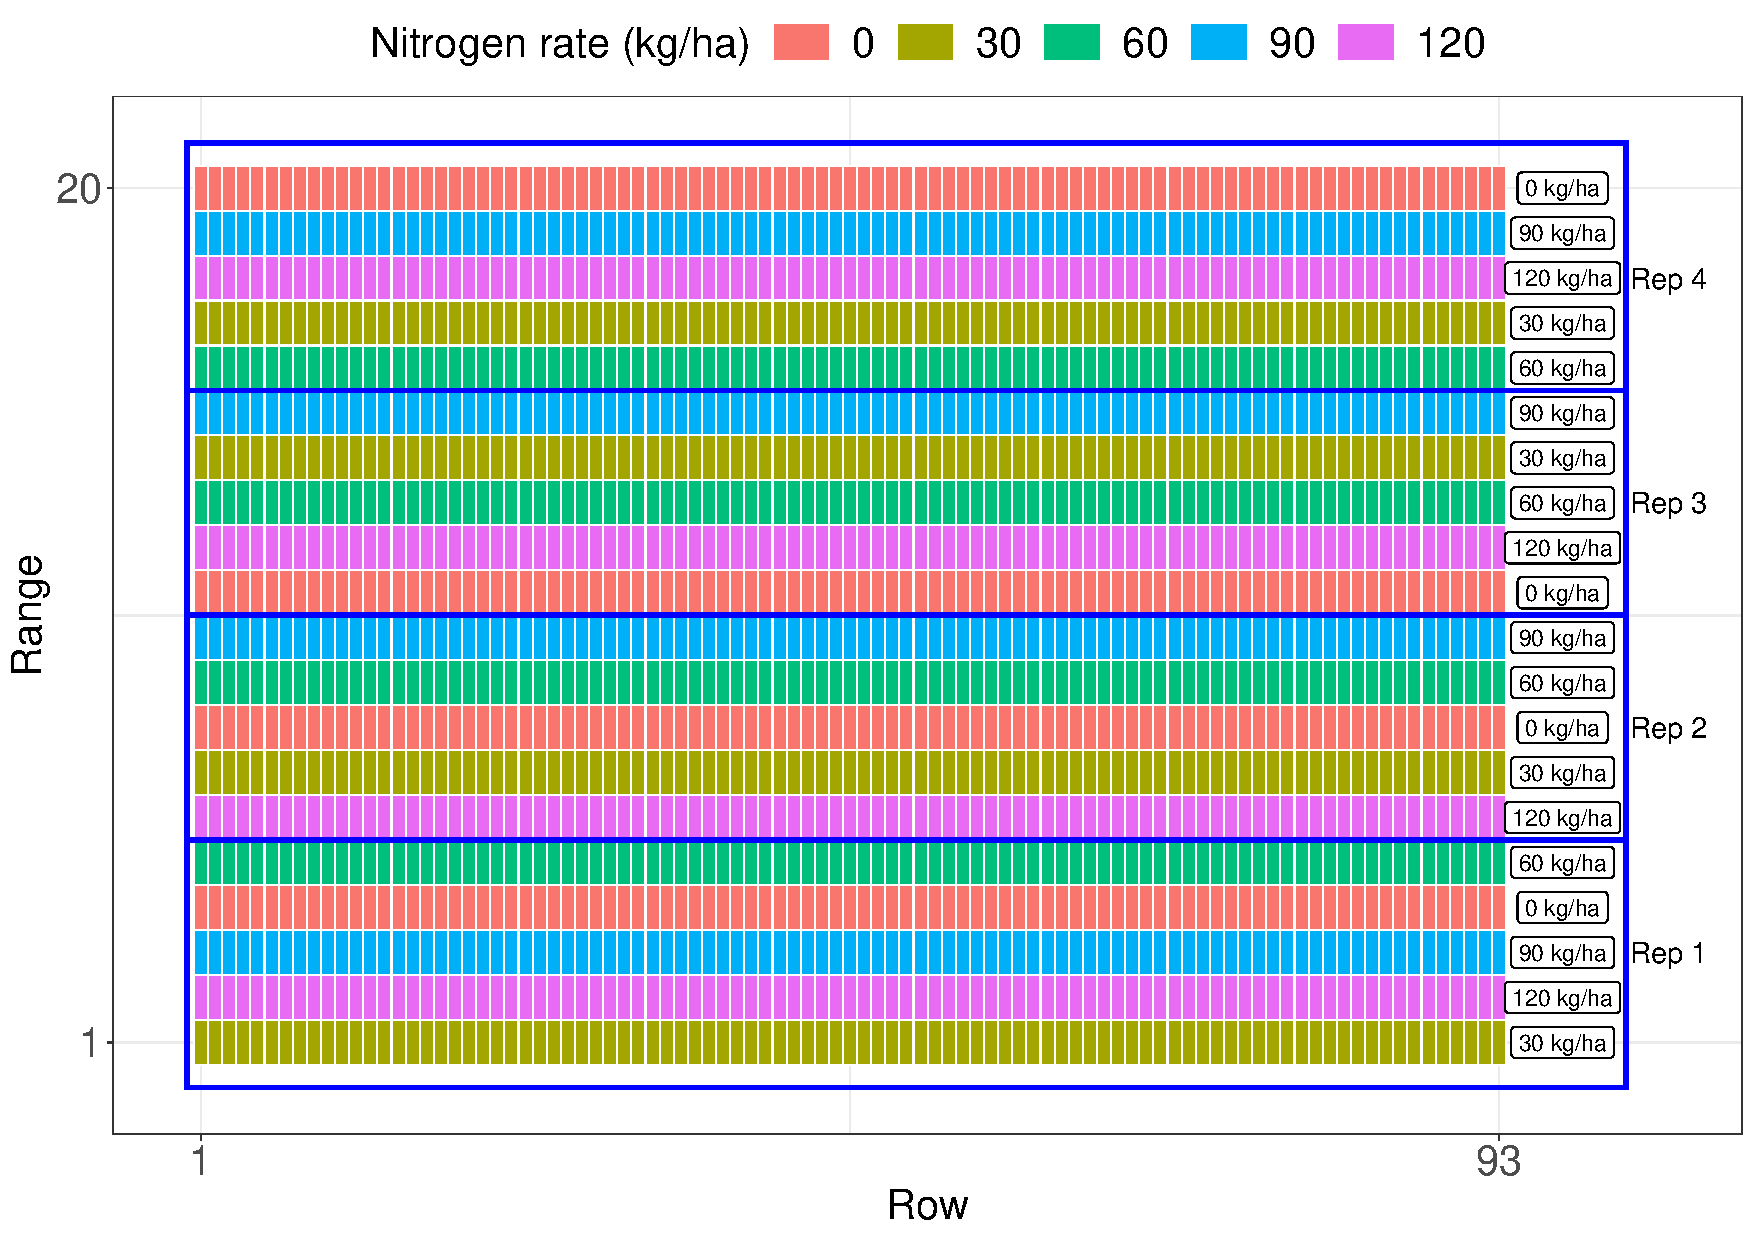
\includegraphics[width=\linewidth]{Col_RandNitro.pdf}
		\caption{Treatments are randomly allocated into large strips in each replicate block.}\label{fig:RandNitrogen}
	\end{subfigure}
	\hspace{0.05\textwidth}
	\begin{subfigure}[t]{0.45\textwidth}
		\centering
		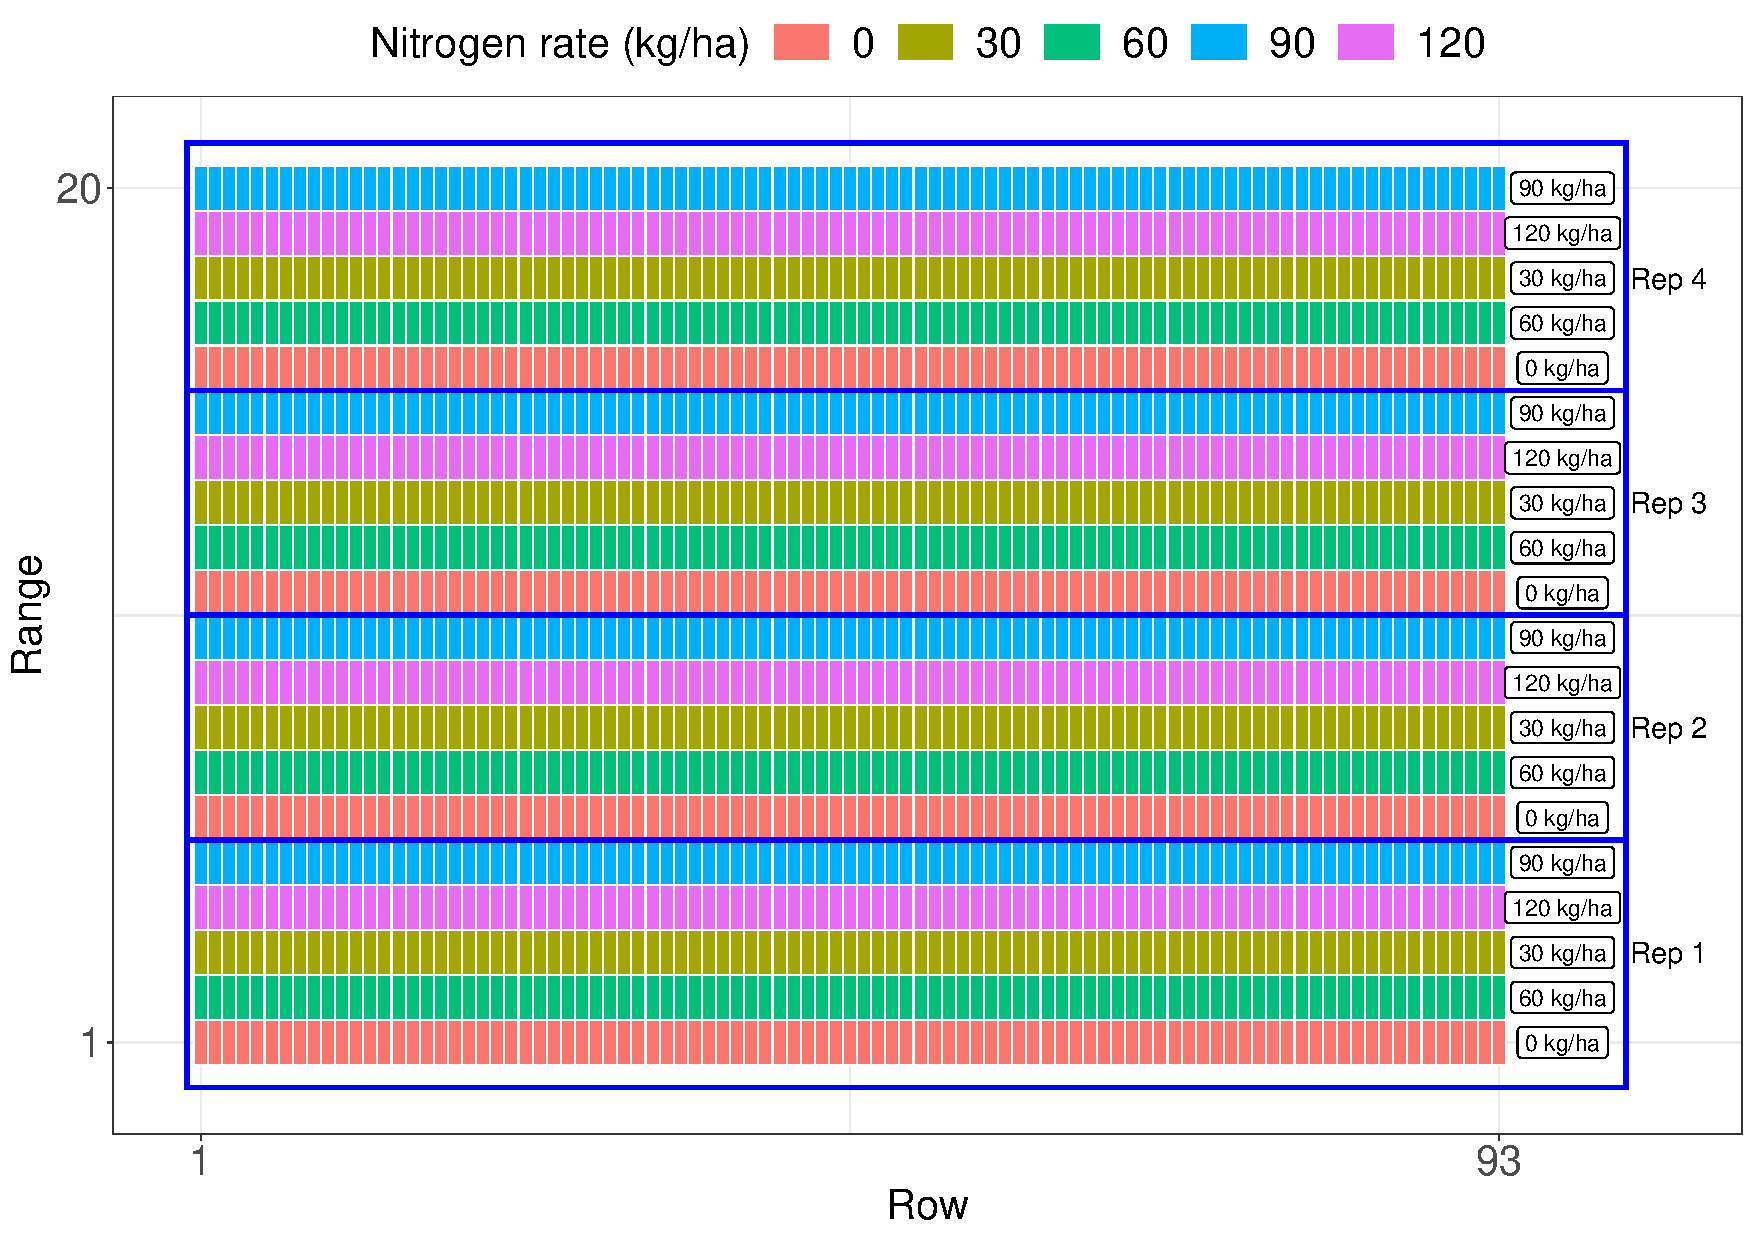
\includegraphics[width=\linewidth]{Col_SystNitro.pdf}
		\caption{Treatments are systematically allocated into large strips in each replicate block.}\label{fig:SystNitrogen}
	\end{subfigure}
	\caption{The nitrogen treatments with five levels (0, 35, 70, 105 and 140 kg/ha) randomly \eqref{fig:RandNitrogen} and systematically \eqref{fig:SystNitrogen} allocated into strips in each replicate block.}\label{fig:Nitrogen}
\end{figure}

With model \eqref{eq:underlying}, the nitrogen rates are treated as continuous observations with five levels. For a linear relationship, we assume that the true global intercept is $b_0 = 65$ and the slope is $b_1=0.05$. The parameters are chosen according to the estimates by \textcite{Rakshit2020Novel, Cao2022Bayesian} on the Las Rosas corn field data, which is initially provided by \textcite{Luc2004ASpatial} and embedded in the \texttt{R}-package \texttt{agridat} \parencite{White2008Agridat}. The unit of yield is quintals per hectare. The variances of $\bm{u}_i$ are $\sigma_{u_0} = 5$ and $\sigma_{u_1}=0.01$. For the $\AR\otimes\AR$ covariance matrix in \eqref{eq:ar1cov}, the two correlation parameters for column and row are $\rho_c = 0.15$ and $\rho_r=0.5$. We have assumed a higher correlation in the rows due to the fact that the crop is traditionally sown and harvested along ranges where the correlation is higher in the perpendicular direction than the travel direction \parencite{Marchant2019Establishinga}. For the \Matern covariance matrix \eqref{eq:matcov}, we set $\sigma_d^2=1$, $r=1$ and $\nu = \frac{3}{2}$. After drawing samples of $\bm{u}$ from $\N(0,\Sigma_u)$, the true spatially varying coefficients are $\bm{\beta}_0 = b_0 + \bm{u}_0$ and $\bm{\beta}_1 = b_1 + \bm{u}_1$. 

Similarly, for the quadratic relationship, we have the true global intercept $b_0 = 65$, coefficients $b_1 = 0.05$ and $b_2 = -0.0003$, 
%where the curve is in a frown shape. 
making the curve concave down. We keep $\sigma_{u_0} = 5$, $\sigma_{u_1}=0.01$ and add $\sigma_{u_2}=0.0001$ because the true values are small. The rest of the parameters remain unchanged. Therefore, the true spatially varying coefficients are $\bm{\beta}_0 = b_0 + \bm{u}_0$, $\bm{\beta}_1 = b_1 + \bm{u}_1$ and $\bm{\beta}_2 = b_2 + \bm{u}_2$.

To summarise, with the true spatially varying coefficients of the treatments, the simulated yield is obtained by 
\begin{equation}
\begin{cases}
	% \text{Linear}  &y_i = b_0 + b_1N_i + u_{0i} + u_{1i}N_i + e_i \\
	\text{Linear}  &y_i = b_0 + u_{0i} + (b_1 + u_{1i})N_i + e_i \\
	% \text{Quadratic} &y_i = b_0 + b_1N_i + b_2N_i^2 + u_{0i} + u_{1i}N_i  + u_{2i}N_i^2 + e_i
	\text{Quadratic} &y_i = b_0 + u_{0i} + (b_1 + u_{1i})N_i + (b_2 + u_{2i})N_i^2 + e_i
\end{cases},
\end{equation}
where $N_i$ is the nitrogen rate, $e_i\sim \N(0,1)$ is the error term at grid $i$, $i = 1, \ldots, n$. Figure \ref{fig:Lines} illustrates how these curves behave for the linear and quadratic relationships.

\begin{figure}[!htp]
	\begin{subfigure}[t]{0.45\textwidth}
		\centering
		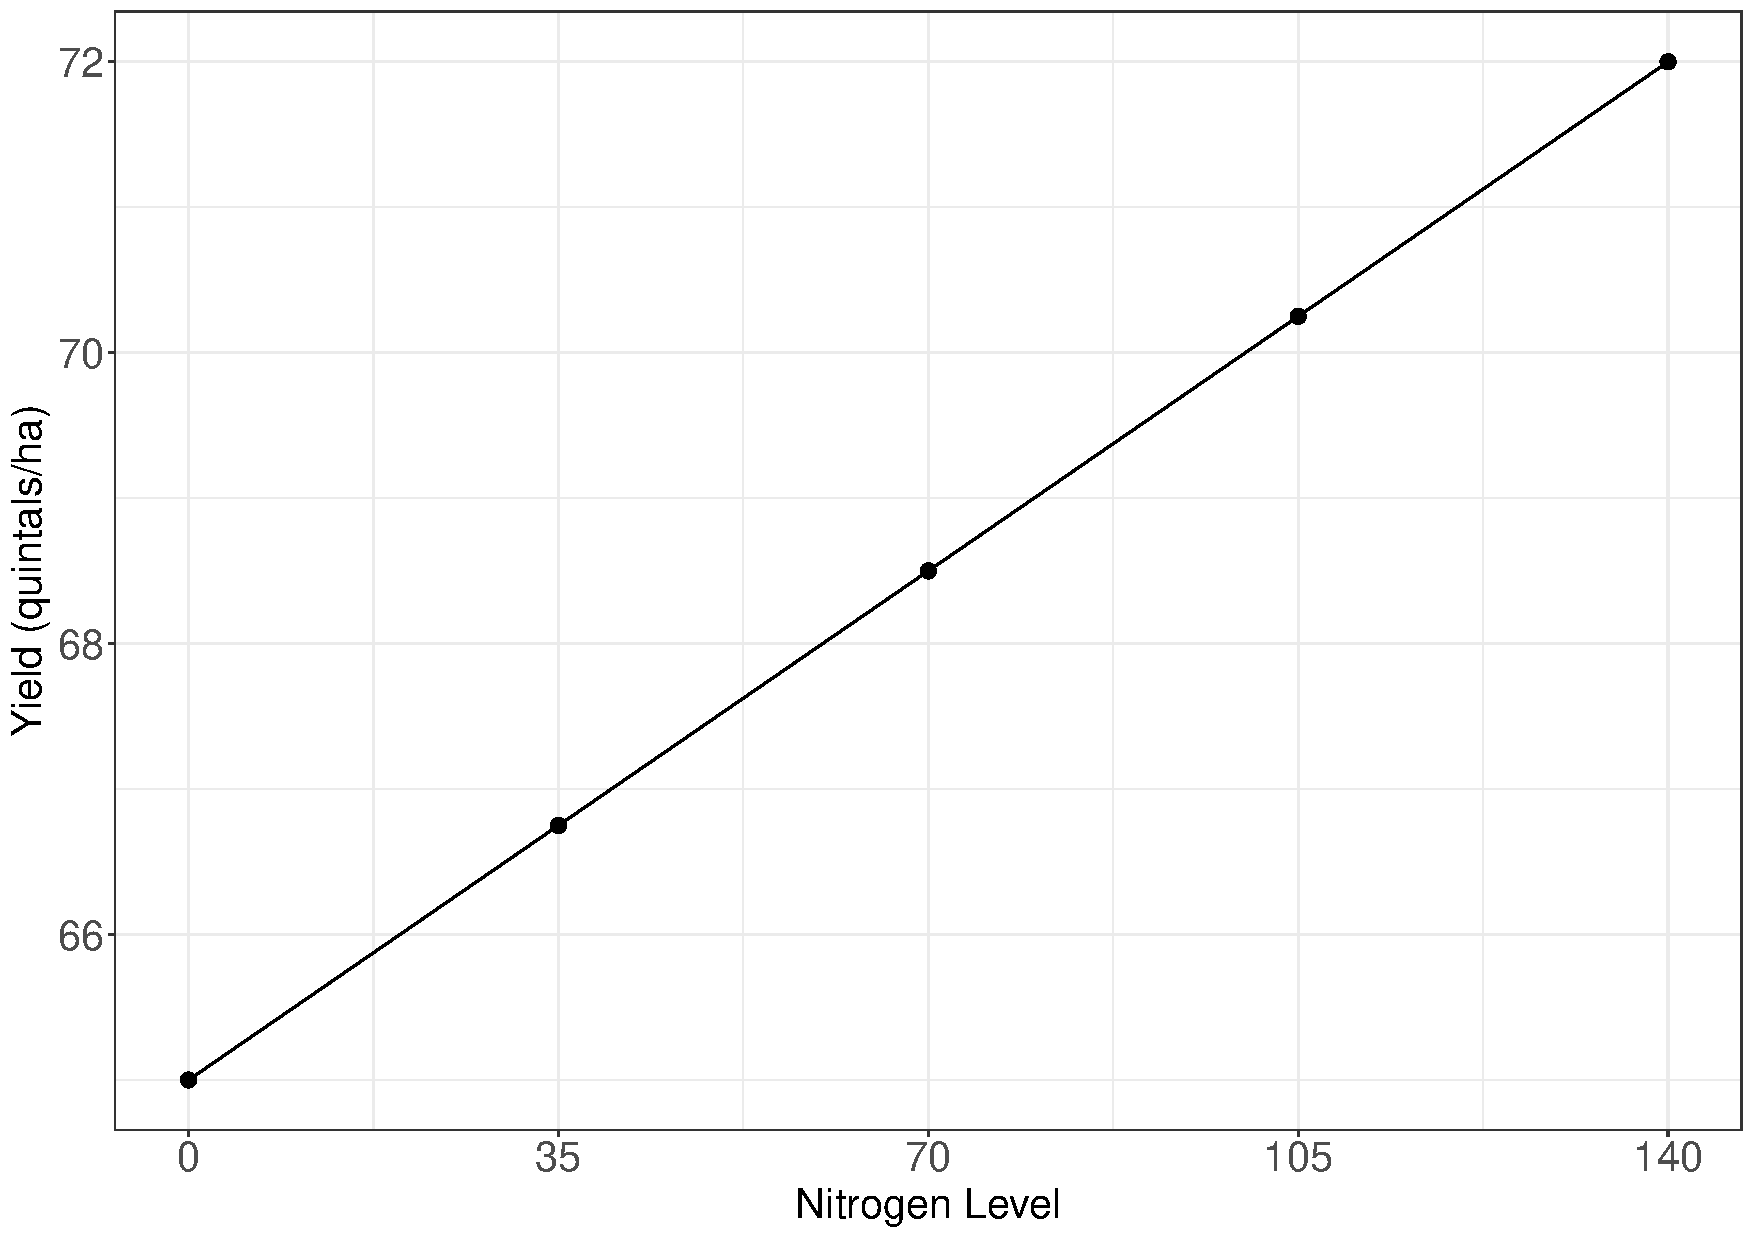
\includegraphics[width=\linewidth]{LinlinesV2.pdf}
		\caption{Linear relationship between crop yield and nitrogen levels, where $y=65+0.05x$.}
	\end{subfigure}
	\hspace{0.05\textwidth}
	\begin{subfigure}[t]{0.45\textwidth}
		\centering
		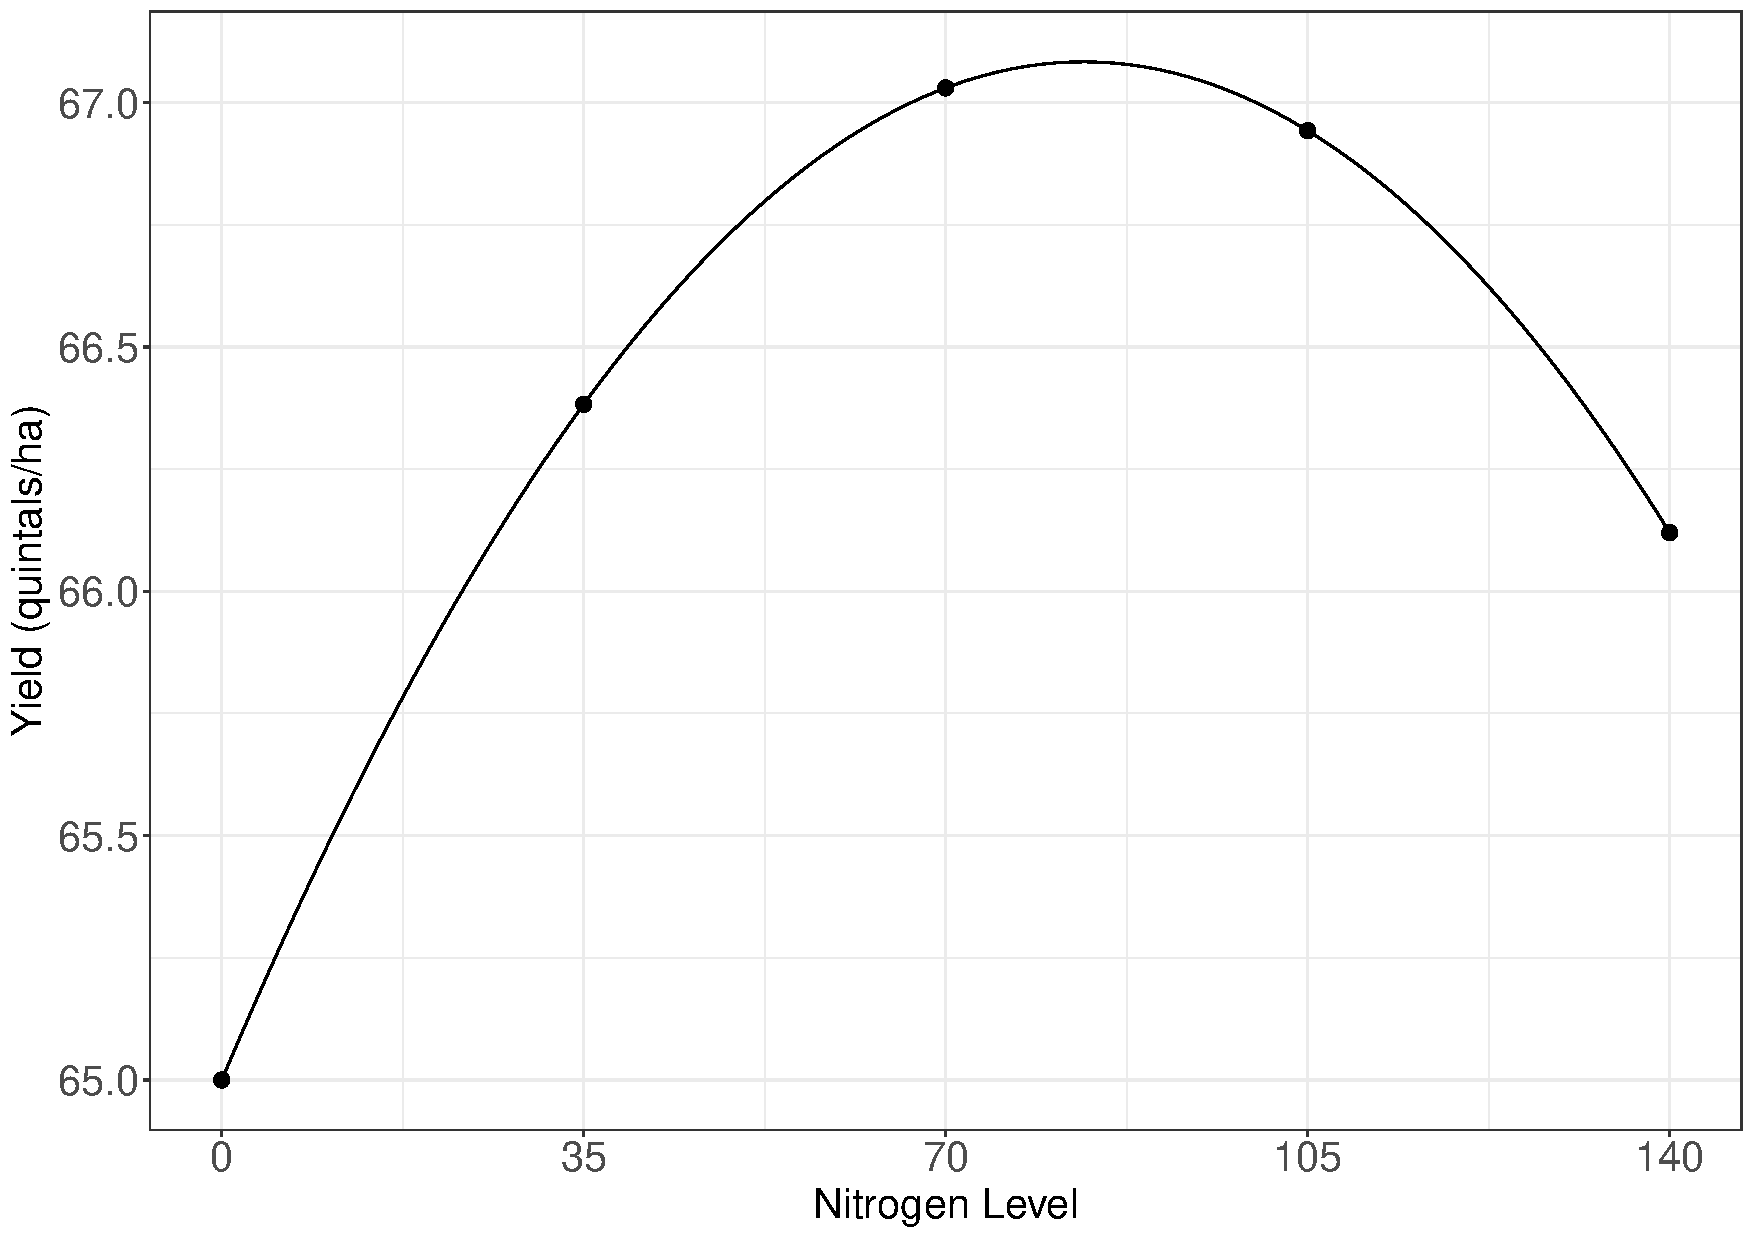
\includegraphics[width=\linewidth]{QualinesV2.pdf}
		\caption{Quadratic relationship between crop yield and nitrogen levels, where $y=65+0.05x-0.003x^2$.}
	\end{subfigure}
	\caption{Noise-free linear and quadratic relationships between crop yield and nitrogen levels.}\label{fig:Lines}
\end{figure}

% Examples of the yield maps with true $\AR\otimes\AR$ spatially varying coefficients are in Figures \ref{fig:LinearYieldMap} and \ref{fig:QuadYieldMap}. 
% \begin{figure}[!htp]
% 	\centering
% 	\begin{subfigure}[t]{0.45\textwidth}
% 		\centering
% 		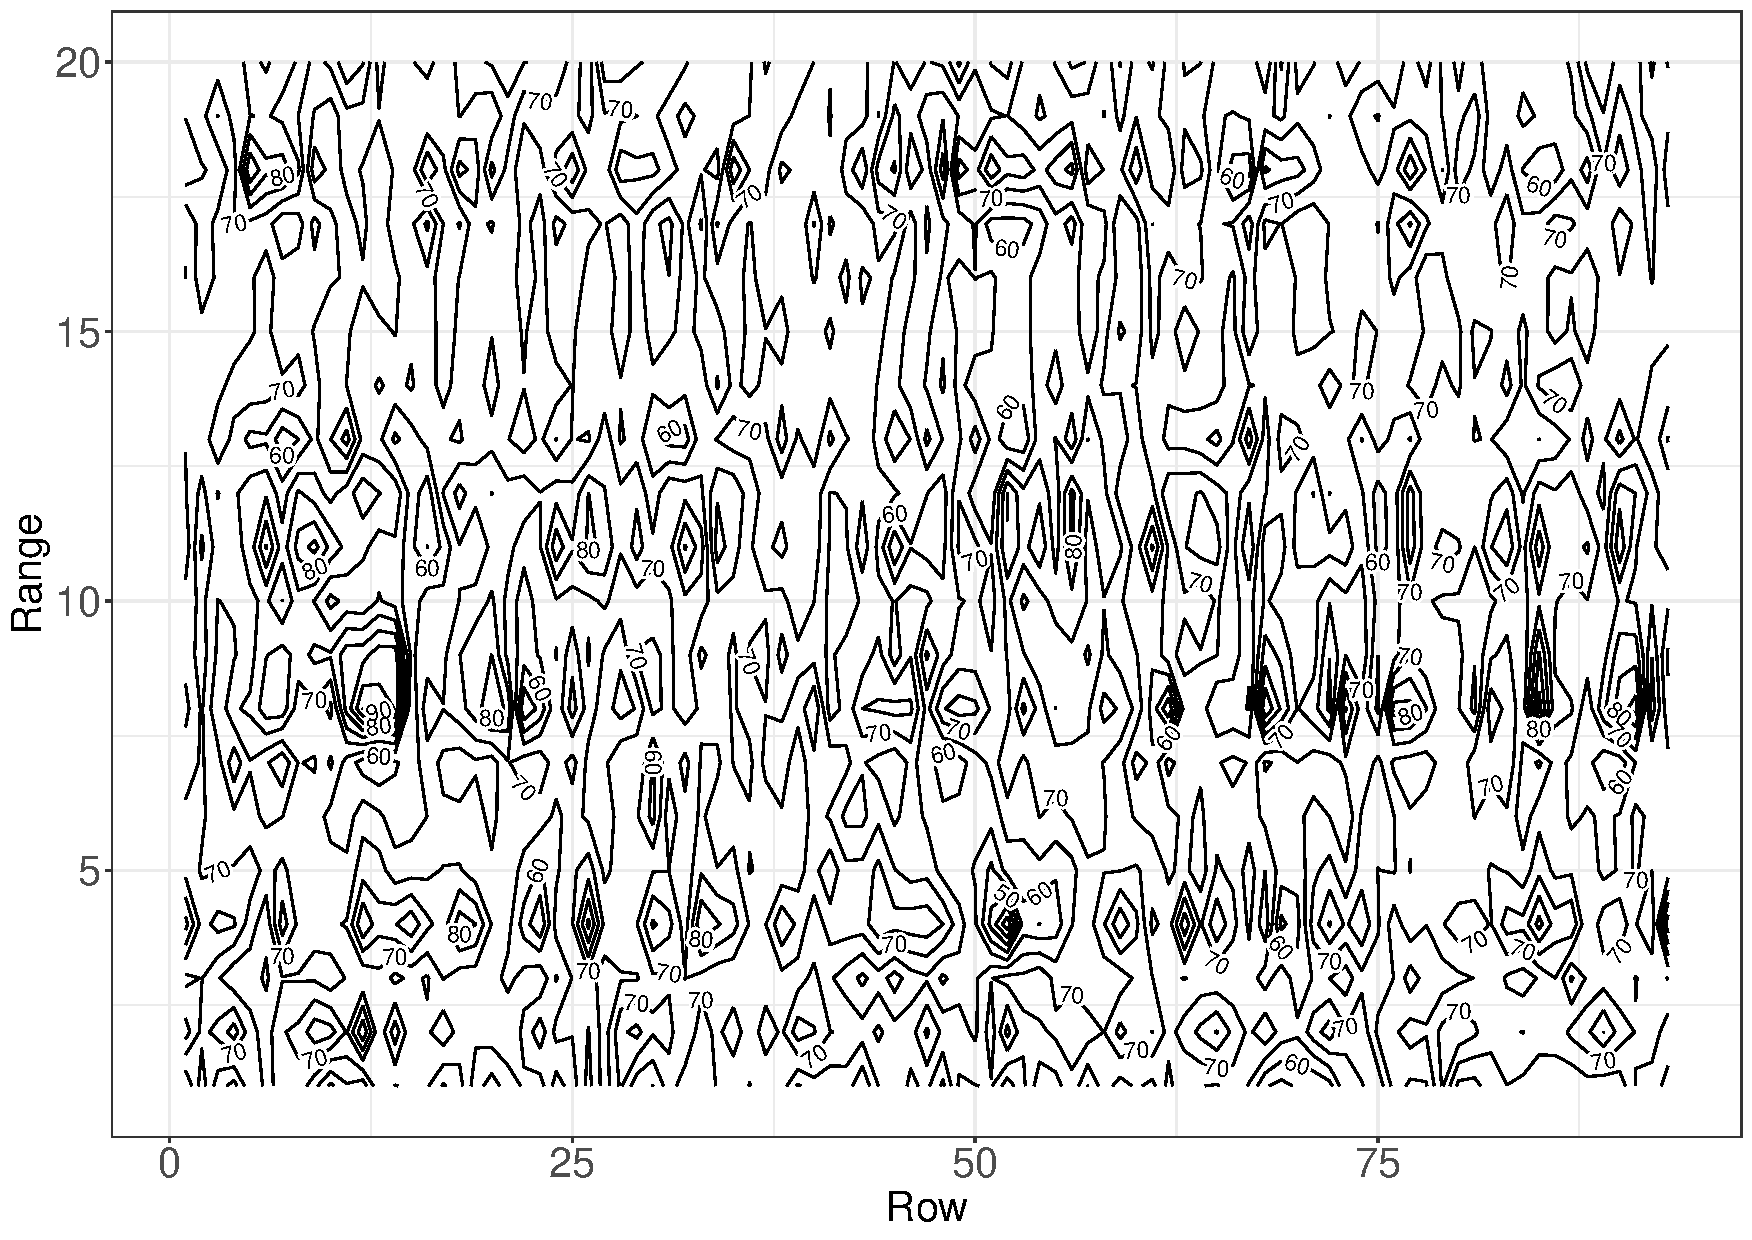
\includegraphics[width=\linewidth]{LinearRandYield01.pdf}
% 		\caption{Yield map of the linear response of the randomised design. }
% 	\end{subfigure}
% 	\begin{subfigure}[t]{0.45\textwidth}
% 		\centering
% 		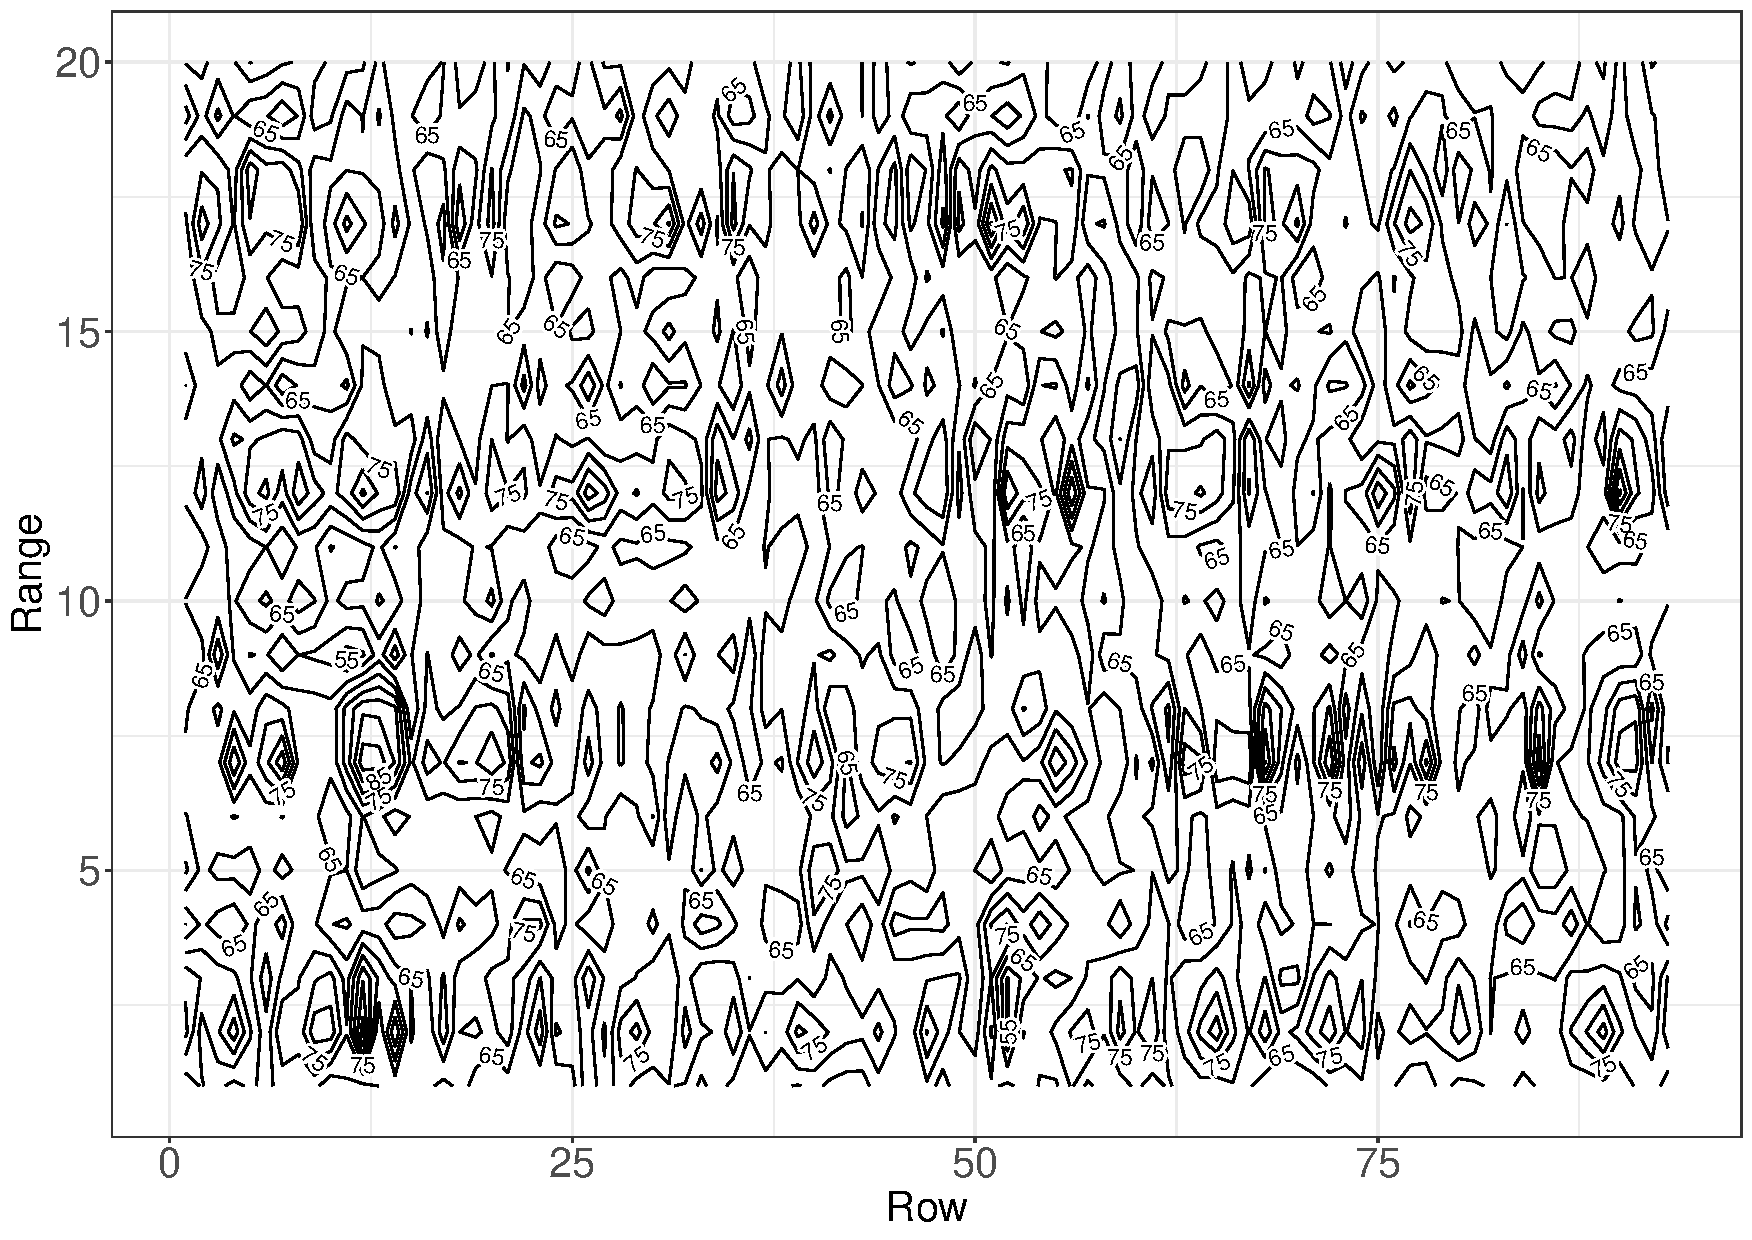
\includegraphics[width=\linewidth]{LinearSystYield01.pdf}
% 		\caption{Yield map of the linear response of the systematic design. }
% 	\end{subfigure}
% 	\caption{Yield maps of linear response of randomly and systematically allocated nitrogen rates.}\label{fig:LinearYieldMap}
% \end{figure}

% \begin{figure}[!htp]
% 	\centering
% 	\begin{subfigure}[t]{0.45\textwidth}
% 		\centering
% 		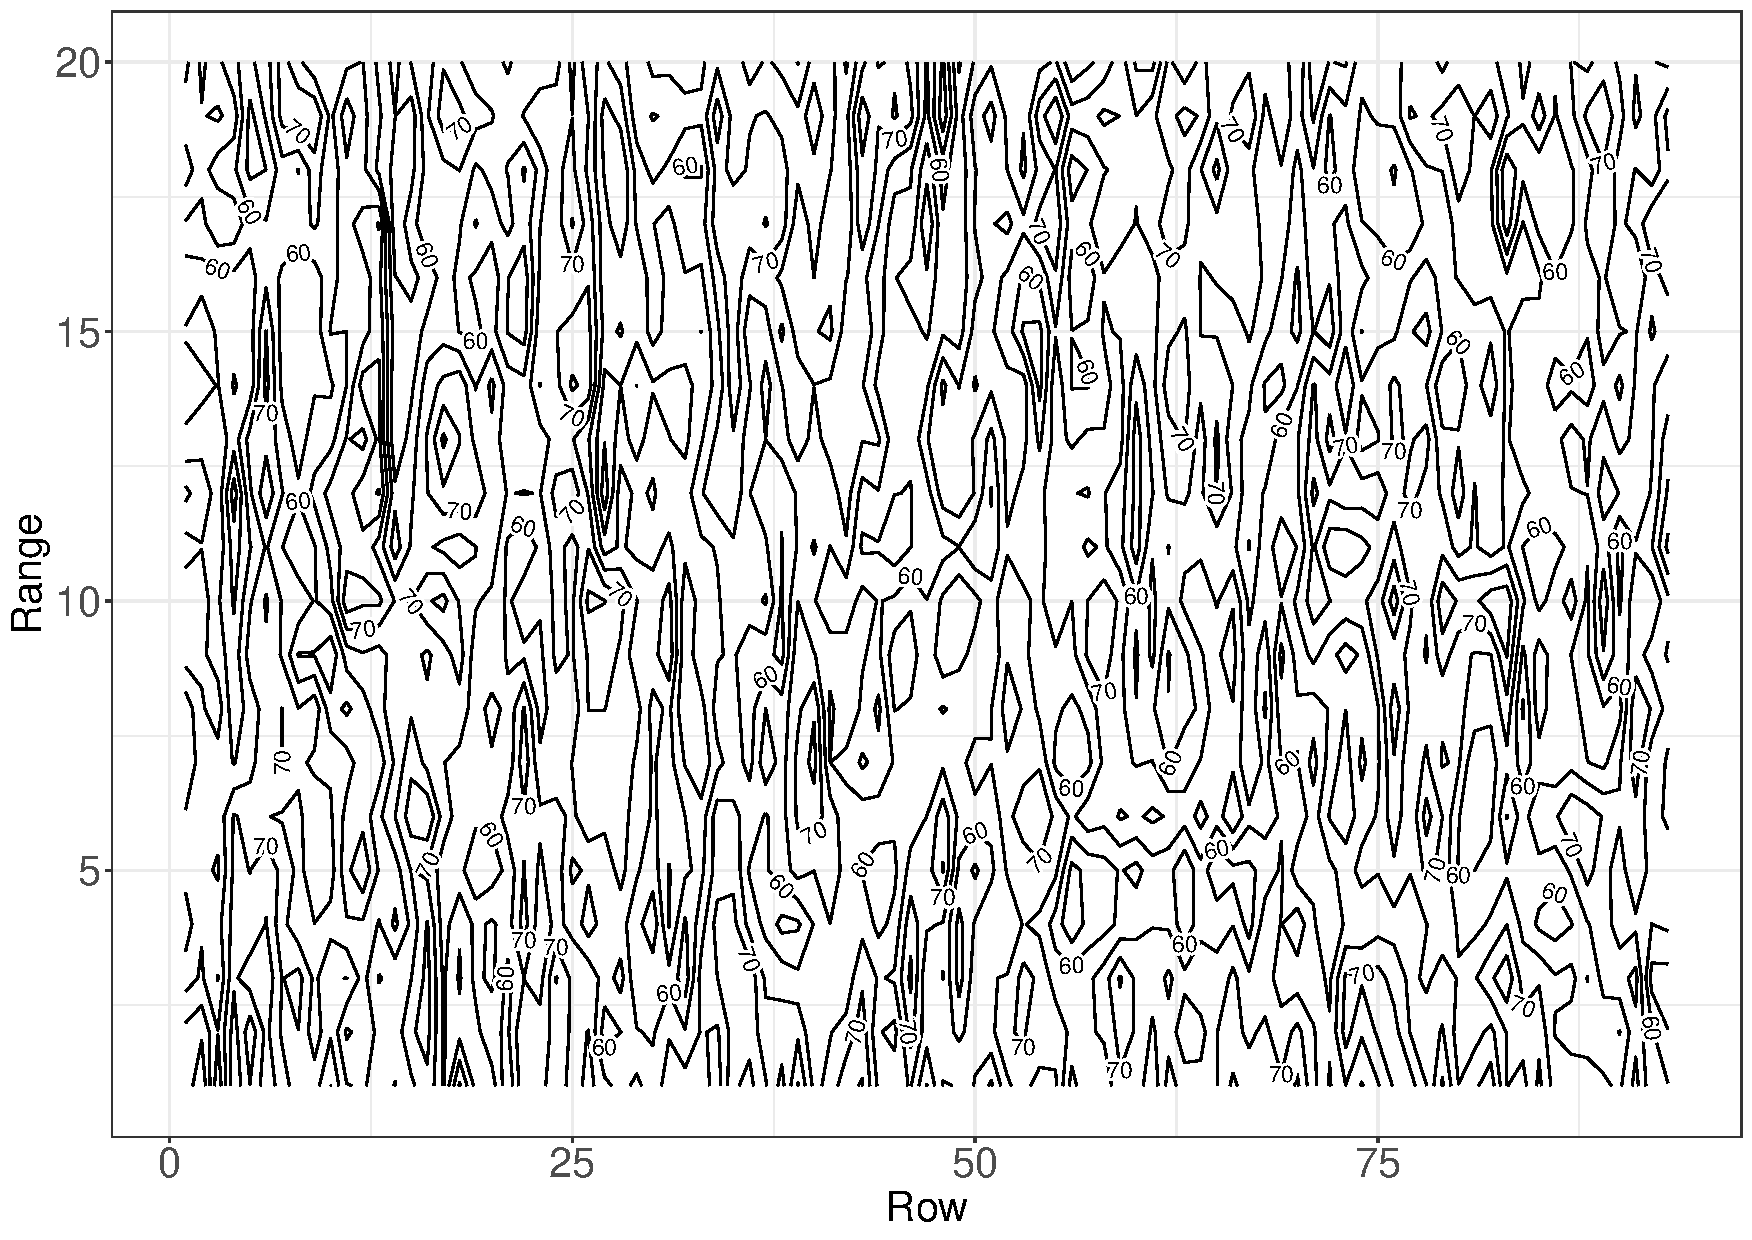
\includegraphics[width=\linewidth]{QuadRandYield01.pdf}
% 		\caption{Yield map of the quadratic response of the randomised design. }
% 	\end{subfigure}
% 	\begin{subfigure}[t]{0.45\textwidth}
% 		\centering
% 		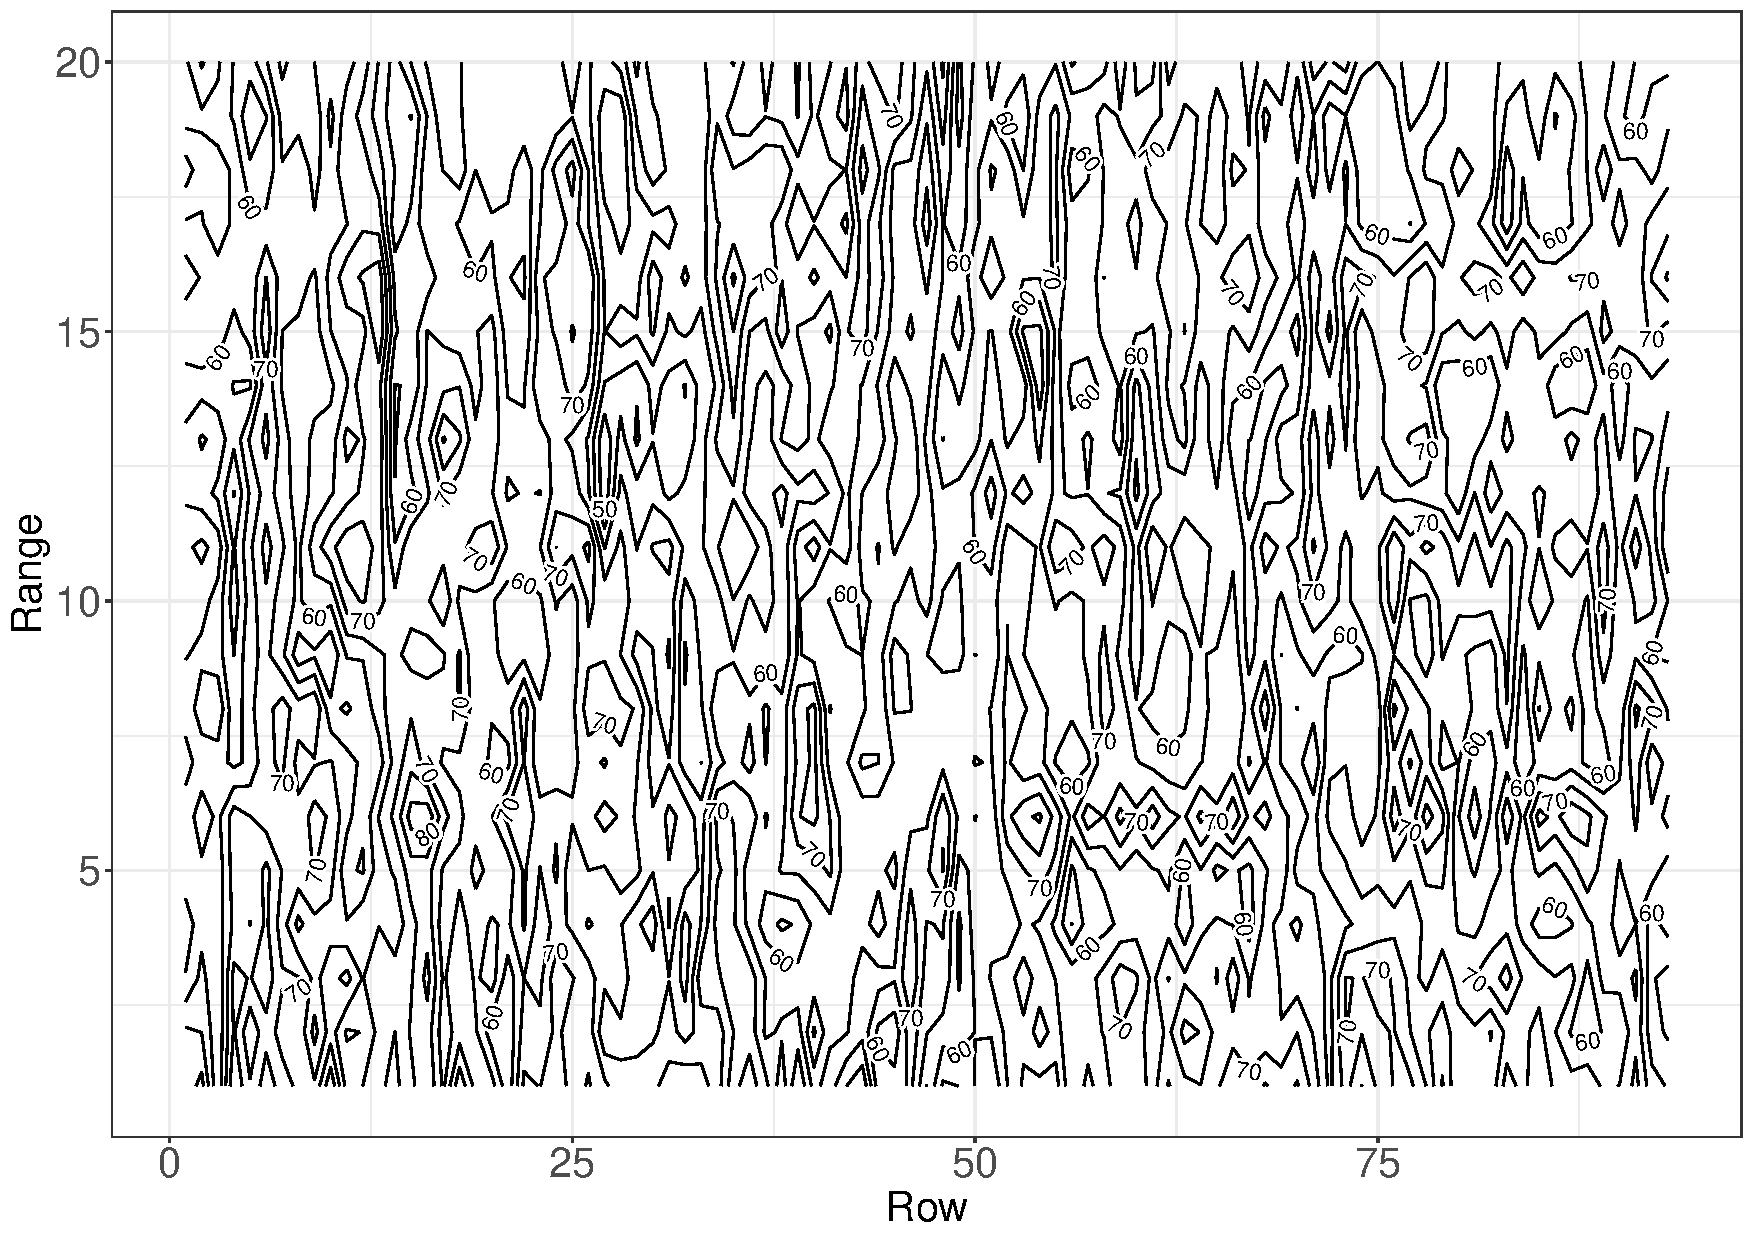
\includegraphics[width=\linewidth]{QuadSystYield01.pdf}
% 		\caption{Yield map of the quadratic response of the systematic design. }
% 	\end{subfigure}
% 	\caption{Yield maps of quadratic response of randomly and systematically allocated nitrogen rates.}\label{fig:QuadYieldMap}
% \end{figure}

%% To fit the data, we use basic GWR with Gaussian kernels. 

The purpose of the simulation study is to test the effect of different types of designs in coefficients estimation by GWR. Identical coefficients were used in one comparison process for two types of designs, and the yield reflects the effect of nitrogen rates.  


\section{Results}\label{Sec:Res}

Running the simulation 100 times, we assessed the performance of the randomised and systematic designs for linear and quadratic responses. In subsection \ref{Sec:MSE} the mean squared errors are compared between the two designs for different bandwidths, parameter correlations and spatial covariance matrices. Subsection \ref{Sec:anova} uses an analysis of variance (ANOVA) test to explore the significance of the factors in the simulation, while subsection \ref{Sec:bandselect} states the performance of bandwidth selection using AICc. 

%By running the simulation 100 times, 

\subsection{Mean squared error}\label{Sec:MSE}

We evaluated the true mean squared error (MSE) of the estimated coefficient differences. This was calculated by the difference of true coefficients, $\bm{\beta} = b + \bm{u}$, and estimated spatially varying coefficients, $\bm{\hat{\beta}} = \hat{b}+\bm{\hat{u}}$, for each grid, and then squared the discrepancy and averaged across the field for comparison. The results are shown in Figures \ref{fig:LinBetaMSE} and \ref{fig:QuadBetaMSE} where ``NS'' stands for no spatial variation ($V_s=I_{n\times n}$), ``AR1'' is for $\AR(0.15)\otimes \AR(0.5)$ and ``Matern'' is the \Matern covariance with $\nu=\frac{3}{2}$. Since the MSEs of $\beta_0$, $\beta_1$, and $\beta_2$ are small, we take the natural logarithm for better visualisation. 

% Paragraph about Figure 3 and the performance for a linear response
With the assumption of a linear response, both randomised and systematic designs perform similarly, meaning GWR is able to partition the local varying intercept and treatment coefficient. Figure \ref{fig:LinBetaMSE} shows that if the response is linear, the MSEs of $\hat{\beta}_0$ and $\hat{\beta}_1$ estimated by GWR, for all bandwidths,
%with bandwidth 5, 9 and the optimal bandwidth found by AICc
is not distinguishing between randomised and systematic designs. This is true regardless of the type of spatial covariance matrix when the correlation within grids is small ($\epsilon=1$), or high ($\epsilon=0.1$) as is shown in Figure \ref{fig:LinBetaMSEeta01}. The GWR with bandwidth selected by AICc has a smaller MSE for its coefficients than the model with a fixed bandwidth (Figure \ref{fig:LinBetaMSE}). 


\begin{figure}[!htp]
	\centering
	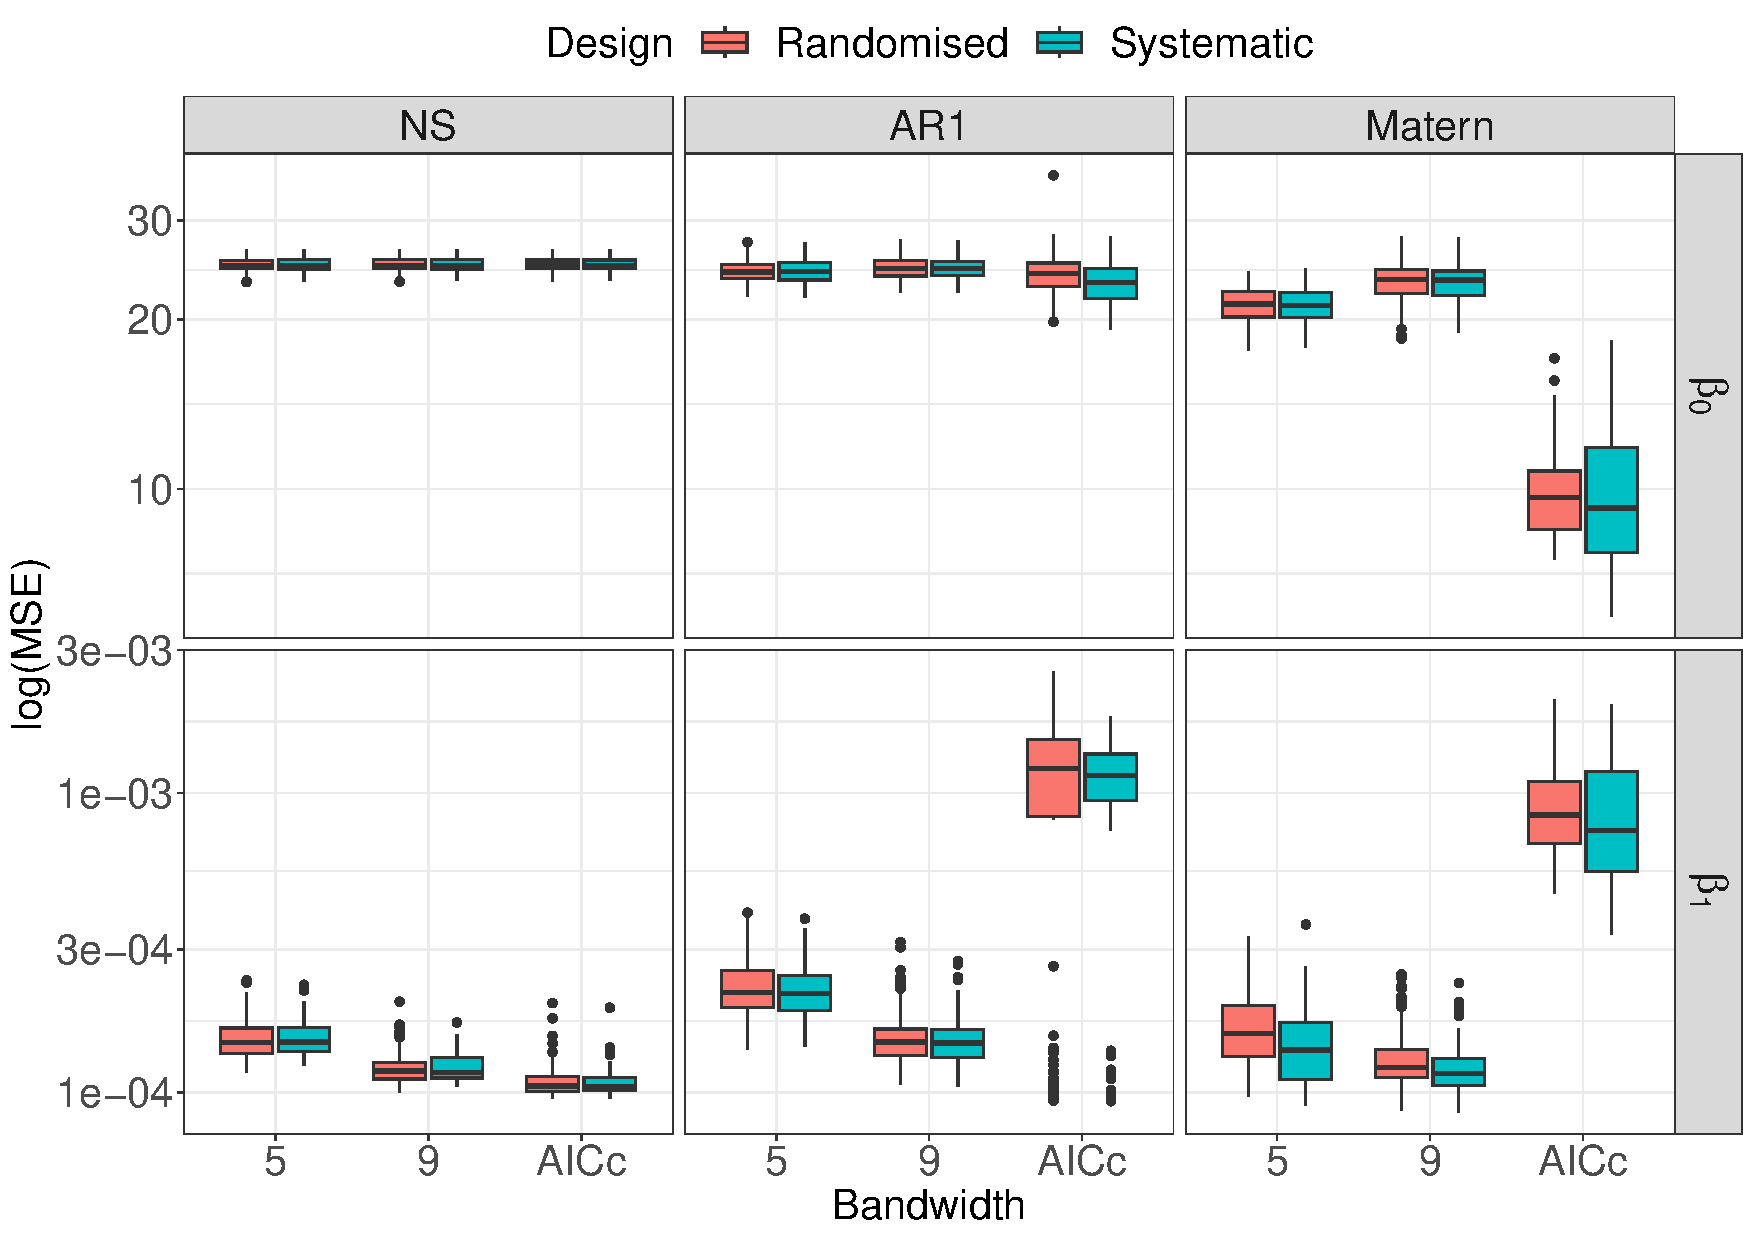
\includegraphics[width=\linewidth]{Col_LinCombMSE_newpar.pdf}
	\caption{Boxplots of the logarithm of MSE for $\hat{\beta}_0$ and $\hat{\beta}_1$ in GWR models using different bandwidths for the simulated data with a linear response. The simulated data had different spatial covariance matrices (NS, AR1$\otimes$AR1 and \Matern) and a low correlation between the parameters ($\epsilon=1$).}\label{fig:LinBetaMSE}
\end{figure}



% Paragraph about Figure 4 and the performance for a linear response
However, if the assumption is a quadratic response, Figures \ref{fig:QuadBetaMSE} and \ref{fig:QuadBetaMSEeta01} show that the GWR with a fixed bandwidth of a systematic design outperforms a randomised design if the spatial correlation is taken into account. With the optimal bandwidth, GWR successfully estimates the global intercepts $\beta_0$ but failed in estimating local varying coefficients $\beta_1$ and $\beta_2$, where the MSE is relatively larger than with fixed bandwidth. However, if we only compare across two types of designs, it still proves that GWR is robust to fit a systematic design rather than a randomised design if the assumption is a quadratic response, regardless of the intensity of the correlation within grids. 

\begin{figure}[!thp]
	\centering
	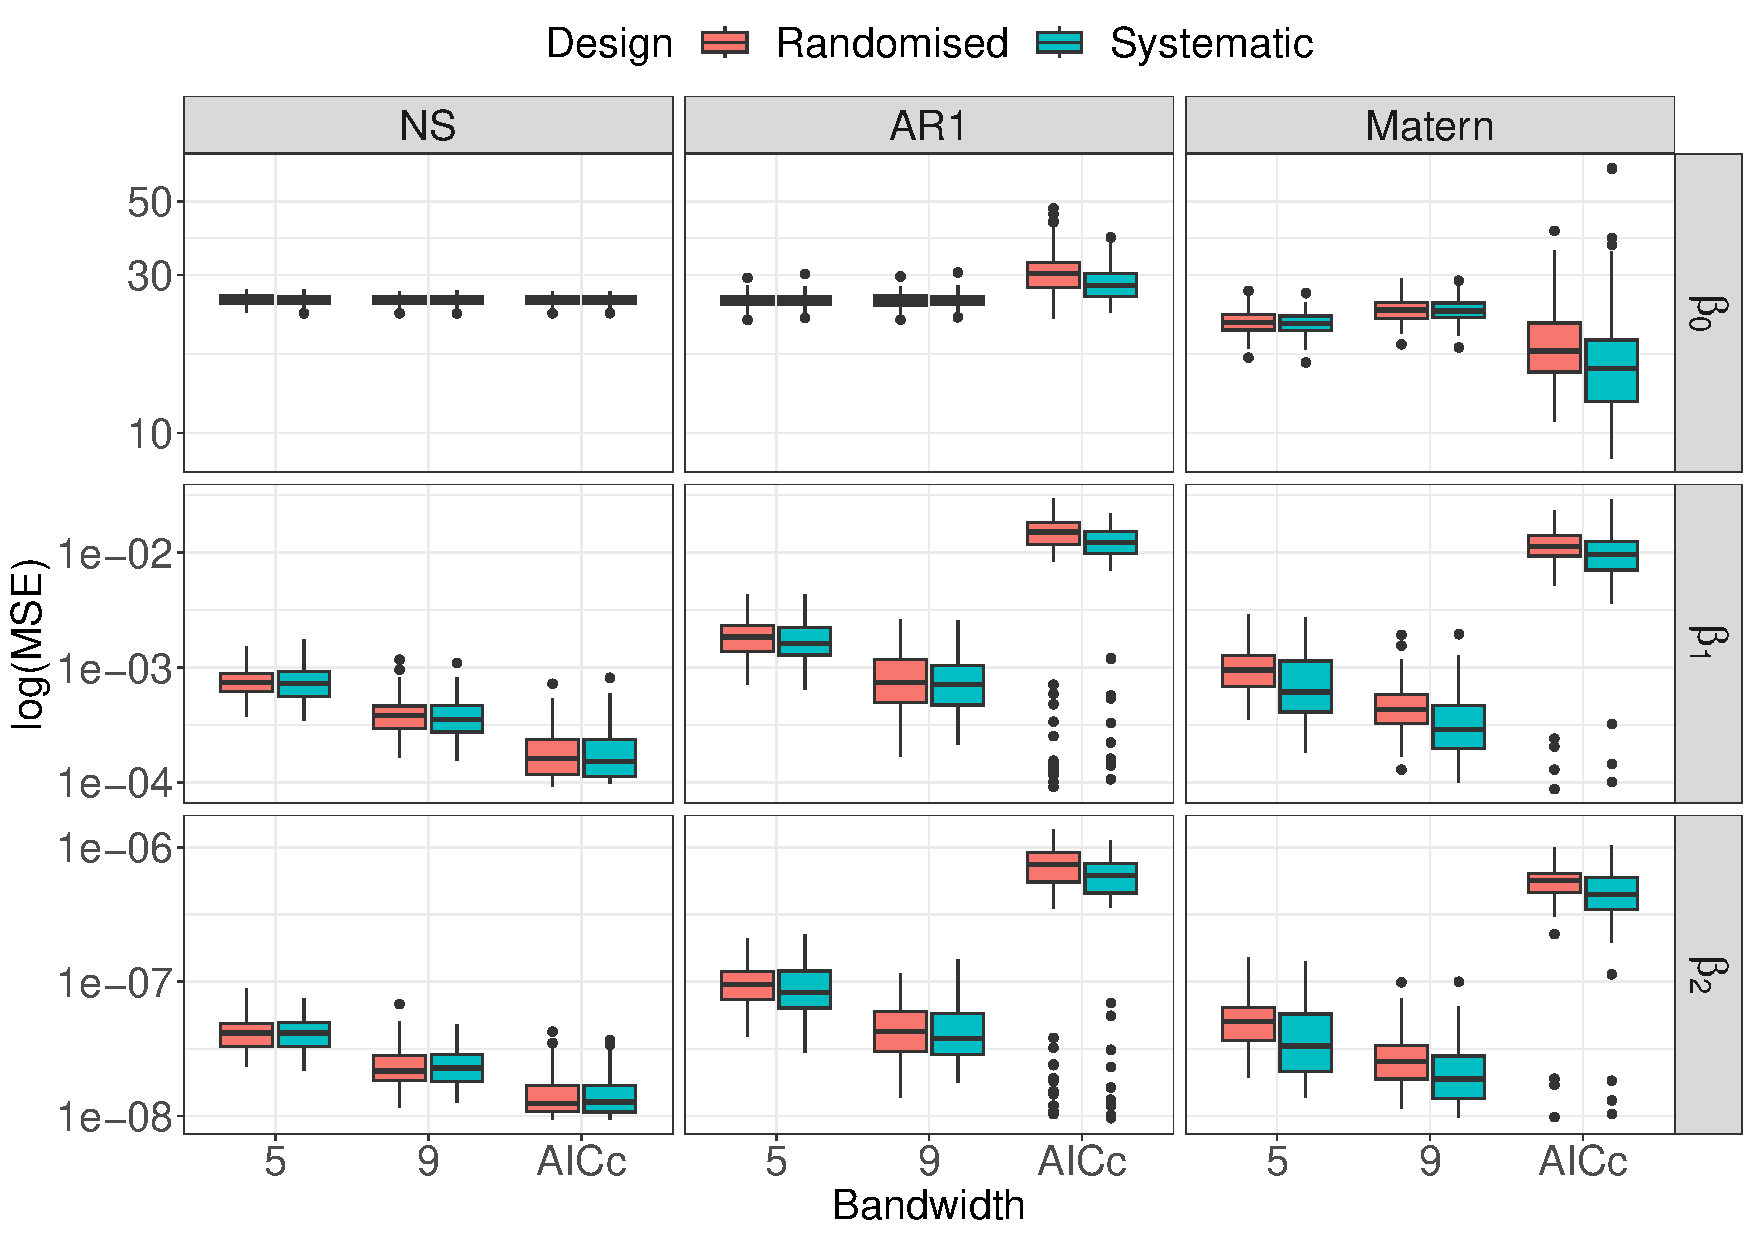
\includegraphics[width=\linewidth]{Col_QuaCombMSE_newpar.pdf}
	\caption{Boxplots of the logarithm of MSE for $\hat{\beta}_0$, $\hat{\beta}_1$ and $\hat{\beta}_2$ in GWR models using different bandwidths for the simulated data with a quadratic response. The simulated data had different spatial covariance matrices (NS, AR1$\otimes$AR1 and \Matern) and a low correlation amongst the parameters ($\epsilon=1$).} \label{fig:QuadBetaMSE}
\end{figure}

% Bandwidth MSE Result

%%The relative MSE for each bandwidth was found to change according to the spatial covariance matrix as well as the coefficient. When no spatial variation was simulated for $\beta_1$ and $\beta_2$, the AICc-selected bandwidth has the lowest MSE, followed by the fixed bandwidths of 9 and then 5. When there is spatial variation (either AR1$\otimes$AR1 or \Matern) present the estimation for $\beta_1$ and $\beta_2$ has the lowest MSEs when using bandwidth 9, followed by 5 and then bandwidth from AICc. The intercept ($\beta_0$) shows only significant changes in MSE amongst the bandwidths when the \Matern spatial covariance was considered. In this case, the bandwidth selected by AICc produces the smallest MSE.

MSE analyses revealed that the choice of bandwidth significantly influenced the relative performance based on both the spatial covariance matrix and the coefficient characteristics. In scenarios without spatial variation for $\beta_1$ and $\beta_2$, the AICc-selected bandwidth demonstrated the lowest MSE, followed by fixed bandwidths of 9 and 5, respectively. However, when the spatial variation was present (utilising either AR1$\otimes$AR1 or \Matern covariance structures), the bandwidth of 9 consistently produced the most accurate estimations for $\beta_1$ and $\beta_2$, outperforming the bandwidths of 5 and the one chosen by AICc. Notably, for the intercept ($\beta_0$), significant changes in MSE amongst the bandwidths were observed only in the context of the \Matern spatial covariance. Here, the bandwidth selected by AICc resulted in the smallest MSE, highlighting its efficacy when dealing with spatially correlated residuals following the \Matern covariance structure. 

Tables \ref{tb:MSElinear} and \ref{tb:MSElinearHigh} are the median MSEs of the linear response for two scenarios: the correlation is low and the correlation is high.

\begin{table}[!htp]
	\centering
\begin{threeparttable}
	\caption{Median MSE of GWR coefficient estimates for a linear response when the correlation between the parameters is low ($\epsilon=1$).}\label{tb:MSElinear}
	\begin{tabular}{llcccccc}
		\toprule
		&  & \multicolumn{3}{c}{Randomised} & \multicolumn{3}{c}{Systematic} \\ 
   		 & Coefficient & 5  &  9  & AICc & 5   & 9  & AICc \\ \midrule
		\multirow{2}{*}{NS}   & $\hat{\beta}_0$ & 24.903 &	24.924 &	24.983&	24.886\tnote{$\dagger$} &	24.911 &	24.965 \\ 
		& $\hat{\beta}_1 (\times 10^3)$ & 0.147&	0.118&	0.105&	0.147&	0.117&	0.104\tnote{$\dagger$}  \\  \midrule
		\multirow{2}{*}{AR1}  & $\hat{\beta}_0$ & 24.308&	24.617&	24.126&	24.319&	24.617&	23.246\tnote{$\dagger$}  \\ 
		& $\hat{\beta}_1 (\times 10^3)$ & 0.215	&0.147	&1.208&	0.214&	0.146\tnote{$\dagger$}	&1.143 \\ \midrule
		\multirow{2}{*}{\Matern} & $\hat{\beta}_0$ & 21.303	&23.566	&9.647&	21.164&	23.526&	9.239\tnote{$\dagger$} \\ 
		& $\hat{\beta}_1 (\times 10^3)$ & 0.157	&0.121&	0.845&	0.138&	0.115\tnote{$\dagger$} &	0.749 \\
		\bottomrule
	\end{tabular}
	\begin{tablenotes}
	\item[$\dagger$] \footnotesize Indicates the smallest MSE for the row.
	\end{tablenotes}
\end{threeparttable}
\end{table}

\begin{table}[!htp]
	\centering
\begin{threeparttable}
	\caption{Median MSE of GWR coefficient estimates of linear response when the correlation between the parameters is high ($\epsilon=0.1$).}\label{tb:MSElinearHigh}
	\begin{tabular}{llcccccc}
		\toprule
		&  & \multicolumn{3}{c}{Randomised} & \multicolumn{3}{c}{Systematic} \\ 
		& Coefficient & 5  &  9  & AICc & 5   & 9  & AICc \\ \midrule
		\multirow{2}{*}{NS}   & $\hat{\beta}_0$  & 24.961	&24.991	&24.958	&24.934\tnote{$\dagger$}	&24.992	&25.020 \\
		& $\hat{\beta}_1 (\times 10^3)$ & 0.144&	0.115&	0.103\tnote{$\dagger$} &	0.145&	0.116&	0.104 \\ \midrule
		\multirow{2}{*}{AR1$\otimes$AR1}  & $\hat{\beta}_0$  & 24.234&	24.518&	23.696&	24.171	&24.497&	23.421\tnote{$\dagger$}  \\
		& $\hat{\beta}_1 (\times 10^3)$   & 0.216	&0.144\tnote{$\dagger$} &	1.024&	0.211&	0.146&	1.027 \\ \midrule
		\multirow{2}{*}{\Matern} & $\hat{\beta}_0$  & 20.882&	22.811&	9.823&	20.770	&22.789	&9.257\tnote{$\dagger$}  \\
		& $\hat{\beta}_1 (\times 10^3)$  & 0.152&	0.120&	0.939&	0.140&	0.112\tnote{$\dagger$} &	0.815 \\ 
		\bottomrule
	\end{tabular}
		\begin{tablenotes}
	\item[$\dagger$] \footnotesize Indicates the smallest MSE for the row.
	\end{tablenotes}
\end{threeparttable}
\end{table}

% \vspace{12pt}

Tables \ref{tb:MSEquadratic} and \ref{tb:MSEquadraticHigh} are the median MSE of the quadratic response for two scenarios: correlation is low and correlation is high. Despite the intensity of the correlation, the data fitted by GWR from systematic designs are superior to randomised designs, in terms of having a lower MSE. 


\begin{table}[!htp]
	\centering
\begin{threeparttable}
	\caption{Median MSE of GWR coefficient estimates of quadratic response when the correlation amongst the parameters is low ($\epsilon=1$).}\label{tb:MSEquadratic}
	\begin{tabular}{llcccccc} \toprule
		 &  & \multicolumn{3}{c}{Randomised} & \multicolumn{3}{c}{Systematic} \\ 
		  & Coefficient & 5  & 9  & AICc & 5  & 9  & AICc \\ \midrule
		\multirow{3}{*}{NS}   & $\hat{\beta}_0$ & 25.218 & 25.150 & 25.152  & 25.263 & 25.179 & 25.138\tnote{$\dagger$}  \\
		& $\hat{\beta}_1 (\times 10^4)$ & 7.417  & 3.823  & 1.625 & 7.233  & 3.529  & 1.516\tnote{$\dagger$}  \\
		& $\hat{\beta}_2 (\times 10^8)$  & 4.157  & 2.168  & 1.242\tnote{$\dagger$} & 4.135  & 2.269  & 1.269   \\ \midrule 
		\multirow{3}{*}{AR1$\otimes$AR1}  & $\hat{\beta}_0$  & 25.185 & 25.092\tnote{$\dagger$} & 30.315  & 25.166 & 25.230 & 27.831  \\
		&$\hat{\beta}_1 (\times 10^4)$  & 18.395 & 7.414  & 151.595 & 16.243 & 7.124\tnote{$\dagger$}  & 123.181  \\
		& $\hat{\beta}_2 (\times 10^8)$ & 9.491  & 4.244  & 74.420  & 8.305  & 3.777\tnote{$\dagger$}  & 61.619 \\ \midrule
		\multirow{3}{*}{\Matern} & $\hat{\beta}_0$  & 21.532 & 23.502 & 17.680  & 21.384 & 23.319 & 15.631\tnote{$\dagger$} \\
		&$\hat{\beta}_1 (\times 10^4)$  & 9.502  & 4.326  & 112.914 & 6.121  & 2.901\tnote{$\dagger$}  & 96.829  \\
		& $\hat{\beta}_2 (\times 10^8)$  & 5.071  & 2.537  & 56.789  & 3.324  & 1.889\tnote{$\dagger$}  & 44.707 \\ \bottomrule
	\end{tabular}
	    \begin{tablenotes}
	        \item[$\dagger$] \footnotesize Indicates the smallest MSE for the row.
	    \end{tablenotes}
\end{threeparttable}
\end{table}

\begin{table}[!htp]
	\centering
\begin{threeparttable}
	\caption{Median MSE of GWR coefficient estimates of quadratic response when the correlation amongst the parameters is high ($\epsilon=0.1$).}\label{tb:MSEquadraticHigh}
	\begin{tabular}{llcccccc} \toprule
		&  & \multicolumn{3}{c}{Randomised} & \multicolumn{3}{c}{Systematic} \\ 
		$\epsilon=0.1$  & Coefficients & 5  & 9  & AICc & 5  & 9  & AICc \\ \midrule
		\multirow{3}{*}{NS} & $\hat{\beta}_0$  & 25.075 & 25.067 & 25.015  & 25.082 & 25.060 & 25.012\tnote{$\dagger$} \\
		&$\hat{\beta}_1 (\times 10^4)$  & 6.683  & 3.466  & 1.478\tnote{$\dagger$} & 7.353  & 3.472  & 1.506 \\
		&$\hat{\beta}_2 (\times 10^8)$  & 3.779  & 2.101  & 1.222\tnote{$\dagger$} & 3.806  & 2.124  & 1.284 \\  \midrule
		\multirow{3}{*}{AR1$\otimes$AR1} & $\hat{\beta}_0$  & 25.103 & 25.223 & 29.266  & 25.033 & 25.032\tnote{$\dagger$} & 27.378 \\
		& $\hat{\beta}_1 (\times 10^4)$ & 16.260 & 6.845  & 130.335 & 16.228 & 6.314\tnote{$\dagger$}  & 112.599  \\
		& $\hat{\beta}_2 (\times 10^8)$  & 8.488  & 3.931  & 61.765  & 7.915  & 3.533\tnote{$\dagger$}  & 54.866  \\  \midrule
		\multirow{3}{*}{\Matern} & $\hat{\beta}_0$ & 21.780 & 23.622 & 18.832  & 21.409 & 23.296 & 15.728\tnote{$\dagger$}  \\
		& $\hat{\beta}_1 (\times 10^4)$ & 11.367 & 5.085  & 122.638 & 6.205  & 2.892\tnote{$\dagger$}  & 88.256 \\
		& $\hat{\beta}_2 (\times 10^8)$  & 5.979  & 2.981  & 60.298  & 3.025  & 1.803\tnote{$\dagger$}  & 43.156  \\ \bottomrule
	\end{tabular}
		    \begin{tablenotes}
	        \item[$\dagger$] \footnotesize Indicates the smallest MSE for the row.
	    \end{tablenotes}
\end{threeparttable}
\end{table}


\subsection{ANOVA}\label{Sec:anova}

Furthermore, ANOVA techniques were used for the analyses of the above results. The analyses were performed for two scenarios of different responses separately. For each response, the coefficients were also taken into account in the model. The objective of the analysis was to investigate the five main factors: two types of design, three bandwidths, three covariance matrices, coefficients $\bm{\beta}$ and correlation $\epsilon$. The significance patterns of the second-order interactions were also of interest. The results are listed in Table \ref{tb:LMMoutput}. 

The results are consistent with what was observed in the previous subsection that, for the linear response, the difference between the randomised and systematic designs was not significant. However, for the quadratic response, the design and its interactions with the bandwidth and the coefficients were significant. For both scenarios, the intensity of the correlation and all its interactions were not significant (Table \ref{tb:LMMoutput}). Therefore, the GWR performs similarly with a low or high correlation between coefficients. Also of note was that bandwidth and its second-order interactions with variables other than correlation were found to be significant for both response types. 

\begin{table}[!htp]
	\centering
	\caption{ANOVA analyses were conducted on the main factors and their second order interactions. The table lists degrees of freedom (Df), sum of squared errors (Sum Sq) and p-values of F tests (Pr($>$F)). }\label{tb:LMMoutput}
	\begin{tabular}{r | lll | lll}
		\toprule
		 & \multicolumn{3}{c|}{Linear}  & \multicolumn{3}{c}{Quadratic}  \\
    & Df & Sum Sq  & Pr(\textgreater{}F) & Df & Sum Sq  & Pr(\textgreater{}F) \\ \midrule 
Design & 1  & 8.46  & 0.0935  & 1  & 74.03 & \textless{}0.001  \\
Bandwidth & 2  & 7453.09 & \textless{}0.001  & 2  & 90.29  & \textless{}0.001  \\
Covariance ($V_s$)  & 2  & 16958.42  & \textless{}0.001  & 2  & 6122.84 & \textless{}0.001 \\
Coefficients ($\beta$)  & 1  & 903705.52 & \textless{}0.001  & 2  & 1419372.21 & \textless{}0.001  \\
Correlation  ($\epsilon$)  & 1  & 5.63  & 0.171   & 1  & 0.07  & 0.8976  \\
Design:Bandwidth  & 2  & 9.21 & 0.216  & 2  & 113.48   & \textless{}0.001  \\
Design:Covariance & 2  & 3.91 & 0.5217  & 2  & 37.55  & 0.0134 \\
Design:Coefficients  & 1  & 8.45 & 0.0935  & 2  & 147.55 & \textless{}0.001  \\
Design:Correlation  & 1  & 0  & 0.9832  & 1  & 0.01  & 0.9541  \\
Bandwidth:Covariance   & 4  & 12283.13  & \textless{}0.001  & 4  & 3135.47  & \textless{}0.001  \\
Bandwidth:Coefficients & 2  & 7456.81 & \textless{}0.001  & 4  & 179.38 & \textless{}0.001  \\
Bandwidth:Correlation  & 2  & 5.95  & 0.3716  & 2  & 0.85  & 0.9073  \\
Covariance:Coefficients  & 2  & 16959.68  & \textless{}0.001  & 4  & 12248.74 & \textless{}0.001  \\
Covariance:Correlation & 2  & 0.26  & 0.9572  & 2  & 11.57  & 0.2649  \\
Coefficients:Correlation & 1  & 5.63  & 0.171   & 2  & 0.15  & 0.9834  \\ \bottomrule  
	\end{tabular}
\end{table}

% For linear response, the type of design is not a key factor that the design and its interactions with other factors are not significant. On the contrary, if the response is quadratic, design becomes a key factor and the interactions are significant as well. For both scenarios, the correlation intensity and most of its interactions are not significant. Hence, either low or high correlation between coefficients works well with GWR. Moreover, bandwidth selection should be based on the design rather than optimality criteria. The results are consistent with the above boxplots. 

\subsection{AICc bandwidth selection}\label{Sec:bandselect}

From the simulation study, we found that the bandwidth given by AICc skewed to 1 if spatial covariance was included in the model, for all types of the design and the nature of the response. If spatial covariance was not introduced, the GWR tended to use all data in one row (Figure \ref{fig:histband}). 

\begin{figure}[!htp]
	\begin{subfigure}[t]{0.45\textwidth}
		\centering
		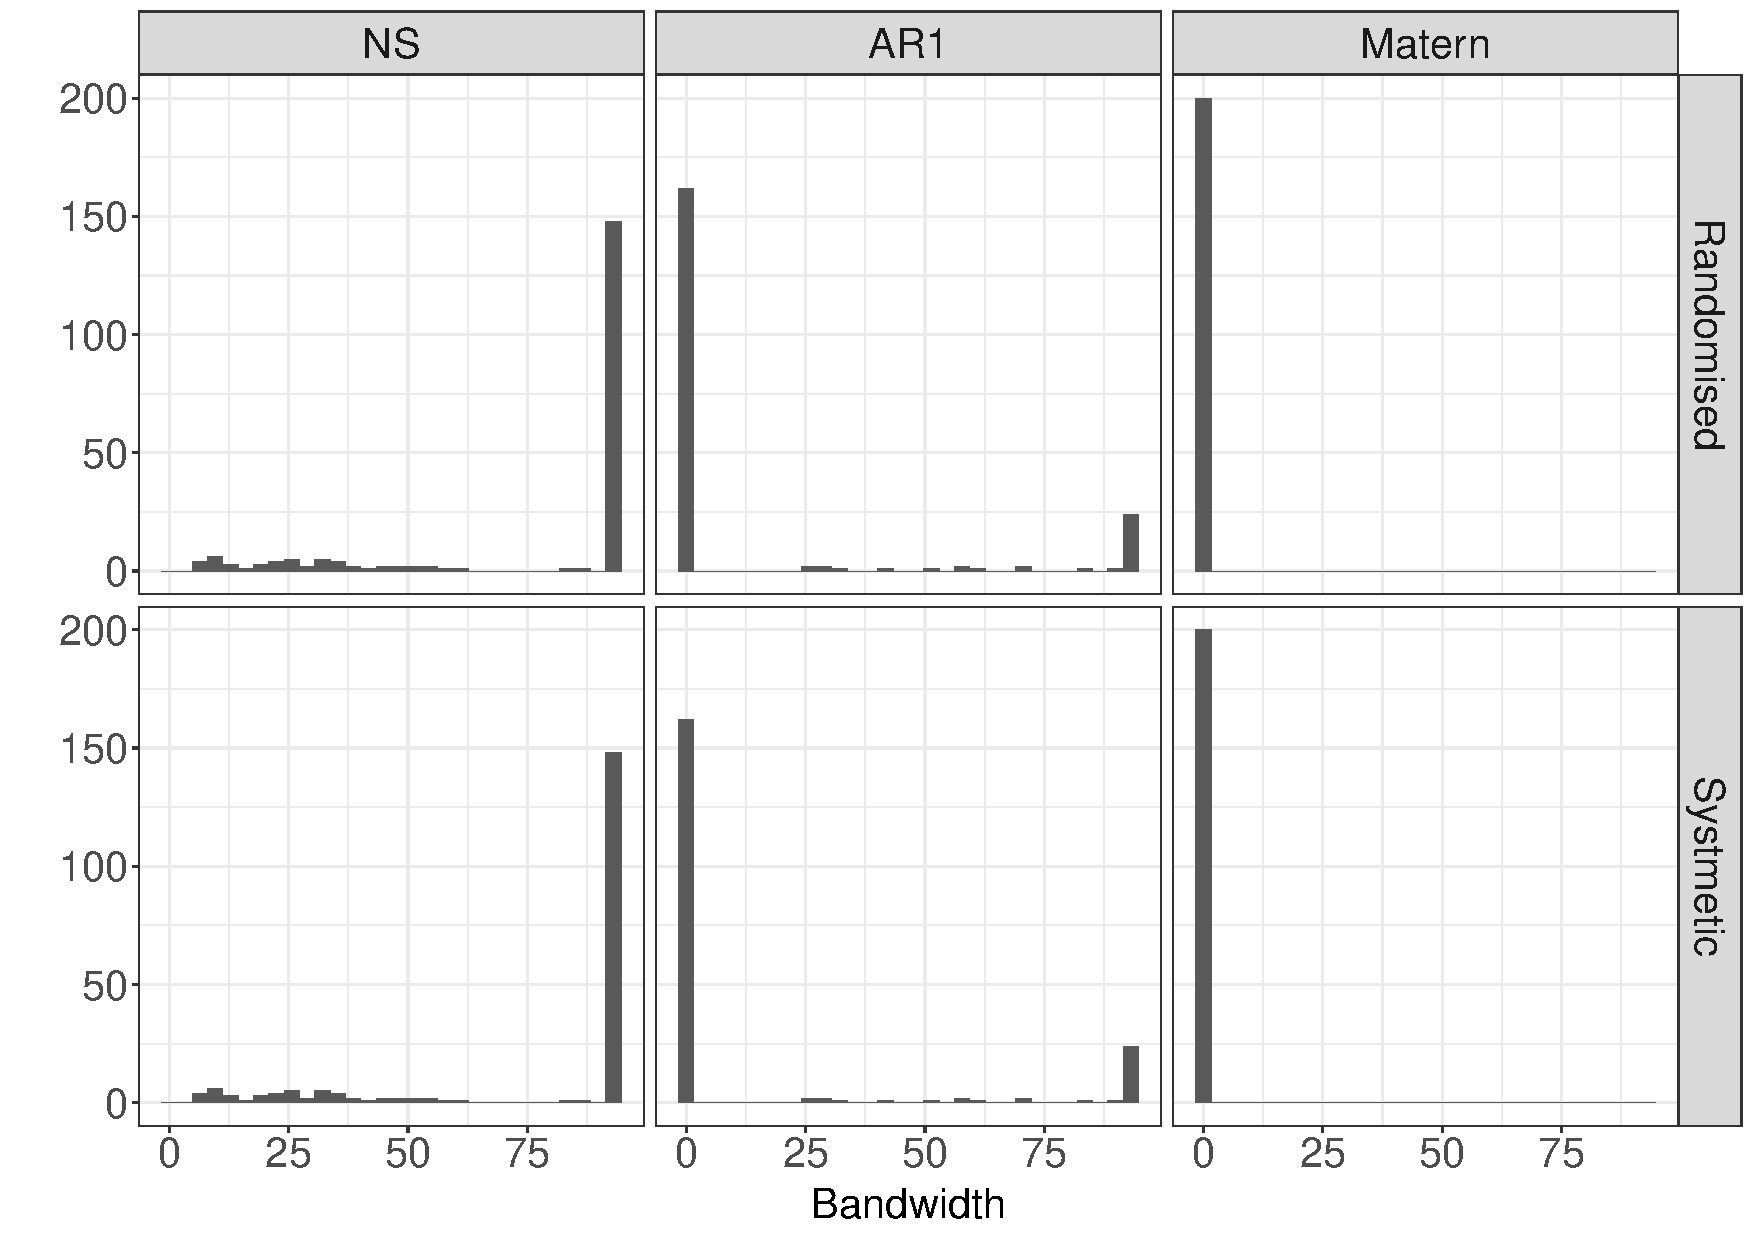
\includegraphics[width=\linewidth]{BandwidthLinear.pdf}
		\caption{Histogram of optimal bandwidth for linear response.}
	\end{subfigure}
	\hspace{0.05\textwidth}
	\begin{subfigure}[t]{0.45\textwidth}
		\centering
		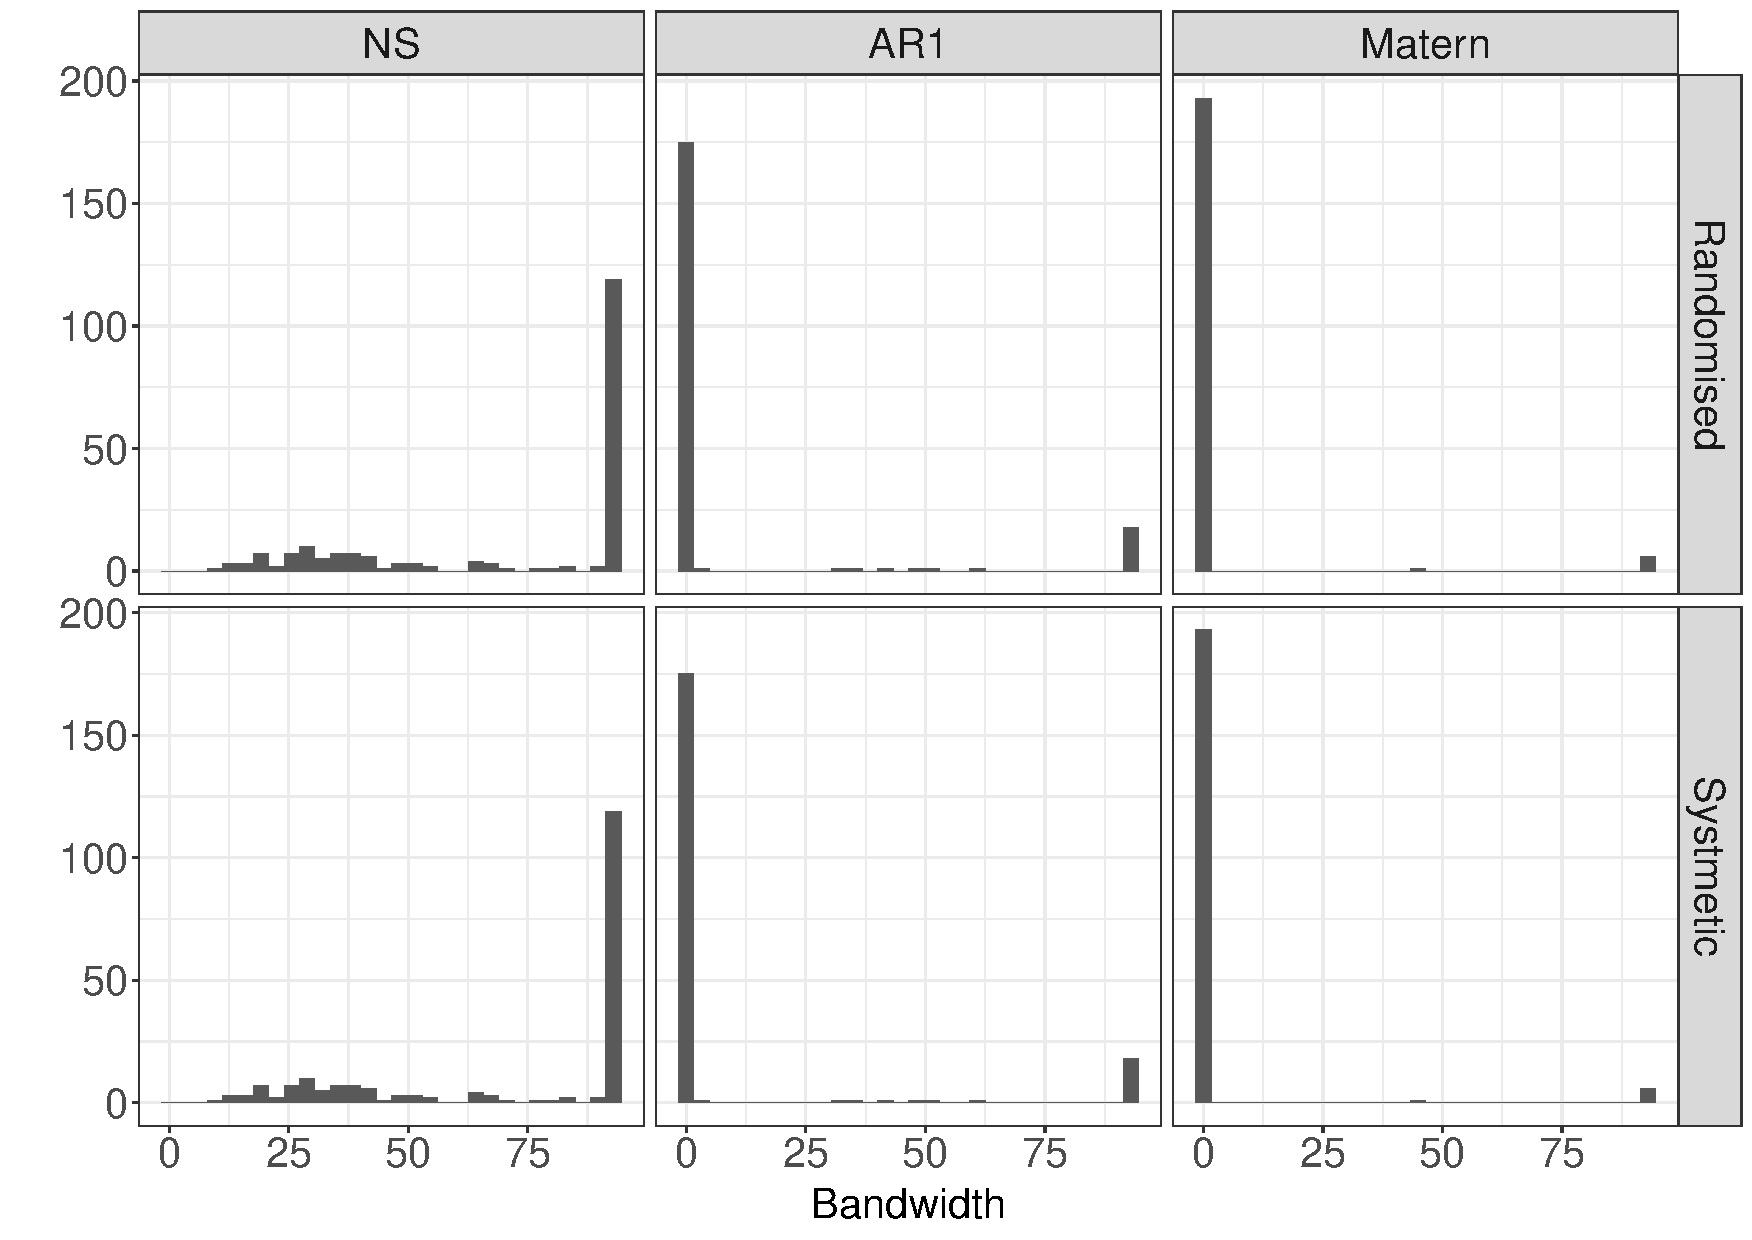
\includegraphics[width=\linewidth]{BandwidthQuadra.pdf}
		\caption{Histogram of optimal bandwidth for quadratic response.}
	\end{subfigure}
	\caption{Histogram of optimal bandwidth found by AICc for linear and quadratic response. }\label{fig:histband}
\end{figure}

\section{Discussion}\label{Sec:Dis}

%1. Summary of Main Findings
Agronomists and biometricians generally prefer randomised designs for OFE trials. According to the performance metrics used, our simulation study shows a systematic design performs either preferably or similarly to a randomised design for the purposes of creating a varying treatment map. The differentiating factors included primarily the response type and the spatial covariance model, while the correlation amongst the treatment coefficients was not found to be important. These are factors that can be assessed by the farmer beforehand, and this should dictate which design should be used. However, given that a systematic design is easier to implement in the field, and shows little downside for the purposes of creating a varying treatment map, we will advocate for the use of systematic designs. 

%2. How response type affected the performance, and what this means
The response type was the main differentiating factor between randomised and systematic designs. When the response was quadratic, the systematic design performed favourably, which contrasted the result for the linear design. Given this, if a farmer expects an approximately linear response in the field, then the selection of the design may not be important. However, given the variable nature of the relationship between response and treatment over a large field (see \textcite{Rakshit2020Novel}), it may be wise to implement a systematic design for the potential outcome of a quadratic relationship. 
%For other more complex response types (i.e polynomials of order greater than 2) it is predicted that a systematic design will also perform favourably. \textcolor{red}{?ref}
%(\textcolor{red}{Might not need a reference)}. 

%2. Discussing Spatial Covariance Structures
%- Some Questions that might be interesting to answer
%- Is a \Matern class more realistic and what are its limitations? %- 
Another consideration for farmers as to which design to use is the expected spatial covariance structure in the field. When no spatial structure was simulated, the differences between the prediction from the systematic and random design were minimal. This result should be expected given that if there are no spatial autocorrelations, then the individual query grids are independent observations, and therefore the design is not important. However, when a first-order auto-regressive structure was simulated, the differences were noticeable when a quadratic response was used, showing systematic designs to be preferential. The largest difference between the two designs occurred when considering the \Matern spatial covariance structure, which showed a clear preference for systematic designs when a quadratic response was considered, and also a small preference for systematic designs for a linear response. Therefore, only if spatial variability was predicted to be negligible in the field would using a randomised design be reasonable given a quadratic response. This assumption of negligible spatial variability would be difficult to reason with given the large fields used in on-farm experimentation (add reference), meaning that in the application a systematic design should be used. 

% Spatial stationarity is seldom the case in small plot research trials even in highly controlled environments. 

%3. Bandwidth selection and why that is important [good]
There were found to be significant deficiencies in using AICc for bandwidth selection. The AICc-minimising bandwidths skewed to 1 and, in a few cases, ended in 93 (number of rows). Even though the bandwidth was optimal according to AICc, the MSE was higher than when using a fixed bandwidth. Therefore, we recommended using the fixed bandwidth based on the experimental design (5 or 9 in this case), rather than the recommended bandwidth from AICc which is prone to either over-fitting or being too generalised. Selecting the bandwidth based on the experimental design is also theoretically better since only a single measurement is observed in each grid, all levels of the treatment factor should be included in a GWR window at the same time to interpolate the %quadratic curve
relationship. Otherwise, the interpolation is incomplete if more than one level is missing. 

% ... AICc-minimising bandwidth were skewed towards the upper ($sqrt(19^2+92^2)=93.94147$) or lower (1) bounds; two characteristics which are suggestive of underlying stationary or random processes  respectively \textcite{}.  
% In this paper, the simulated data is fitted by GWR, which has been proven to accurately separate treatment from non-treatment influence of yield response. One crucial factor of GWR is bandwidth selection. The AICc-minimising bandwidths skew to 1 and, in a few cases, end in 93 (number of rows). Thus, even though the bandwidth is optimal, the MSE is higher than when using a fixed bandwidth. Therefore, we would use the fixed bandwidth of 5 and 9 based on the experimental design, rather than the recommended bandwidth from AICc. Selecting the bandwidth based on the experimental design is also theoretically better. Since only a single measurement is observed in each grid, all levels of the treatment factor should be included in a GWR window at the same time to interpolate the quadratic curve. Otherwise, the interpolation is incomplete if more than one level is missing. 

%4. Paragraph on Coefficient importance (or the lack thereof)
%The level of correlation between the coefficients as governed by $\epsilon$ was found to no be significant (Table \ref{tb:LMMoutput}). This indicates that GWR performs similarly with either low or high correlation between coefficients. %This is an unexpected/expected result... 

%5. Recommendation of design variations
Given the scope of the paper, some designs and factors were not considered. Designs such as chequerboard or wave designs have been suggested for on-farm experiments \parencite{bramley1999designing}, however, were not considered here. Topographical factors (spatial zones) were also not entertained in our study. Since GWR estimates a global template model and then adjusts it at a local scale across the study region, the variation between zones is ``flushed out'' by the spatial covariance.

%However, this is not practical for farmers as the complex layout of the treatments will increase the cost of sowing and harvesting. Therefore, unless the objective is for variety selection, we do not recommend such designs to agronomists. 

%6. Recommendation of other spatial factors to consider, and why those were ignored. 
%Topographical factors (spatial zones) were also not considered in our study. Since GWR estimates a global template model and then adjusts it at a local scale across the study region, the variation between zones is ``flushed out'' by the spatial covariance.

\section{Conclusion}\label{Sec:Conclusion}

Agronomists and biometricians generally prefer randomised designs for OFE trials. With the purpose of creating a varying treatment map, our simulation study proves that a systematic design produces better performance metrics, under particular circumstances, than a randomised design for large on-farm trials in terms of robustness and smaller MSE on coefficients. On the other hand, if spatial variation is not considered or if researchers believe in linear response, a systematic or a randomised design could be implemented because the difference is not significant. We recommend that, for a large OFE strip trial with the goal to create a varying treatment map, a systemic design should be used as it has more flexibility in post-experiment statistical modelling. 

% Perhaps we add a comment along the lines - "Further research is needed in the case of OFE (and GWR?) when it comes to more complex designs such as chequerboard, donut etc."

\section*{Acknowledgements}

Curtin Biometry and Data Analytics (CBADA) gratefully acknowledges the support from the Grains Research and Development Corporation of Australia (GRDC).

\section*{CRediT authorship contribution statement}

\textbf{Zhanglong Cao}: Conceptualization; Formal analysis; Methodology; Software; Validation; Visualization; Roles/ Writing - original draft; and Writing - review \& editing. \textbf{Jordan Brown}: Investigation; Methodology; Visualization; Roles/Writing - original draft; and Writing - review \& editing. \textbf{Mark Gibberd}: Project administration; Roles/Writing - original draft; and Writing - review \& editing. \textbf{Julia Easton}: Roles/Writing - original draft; and Writing - review \& editing. \textbf{Suman Rakshit}: Conceptualization; Methodology; Supervision; Roles/Writing - original draft; and Writing - review \& editing. 


\appendix

\section{Figures}

\begin{figure}[H]
	\centering
	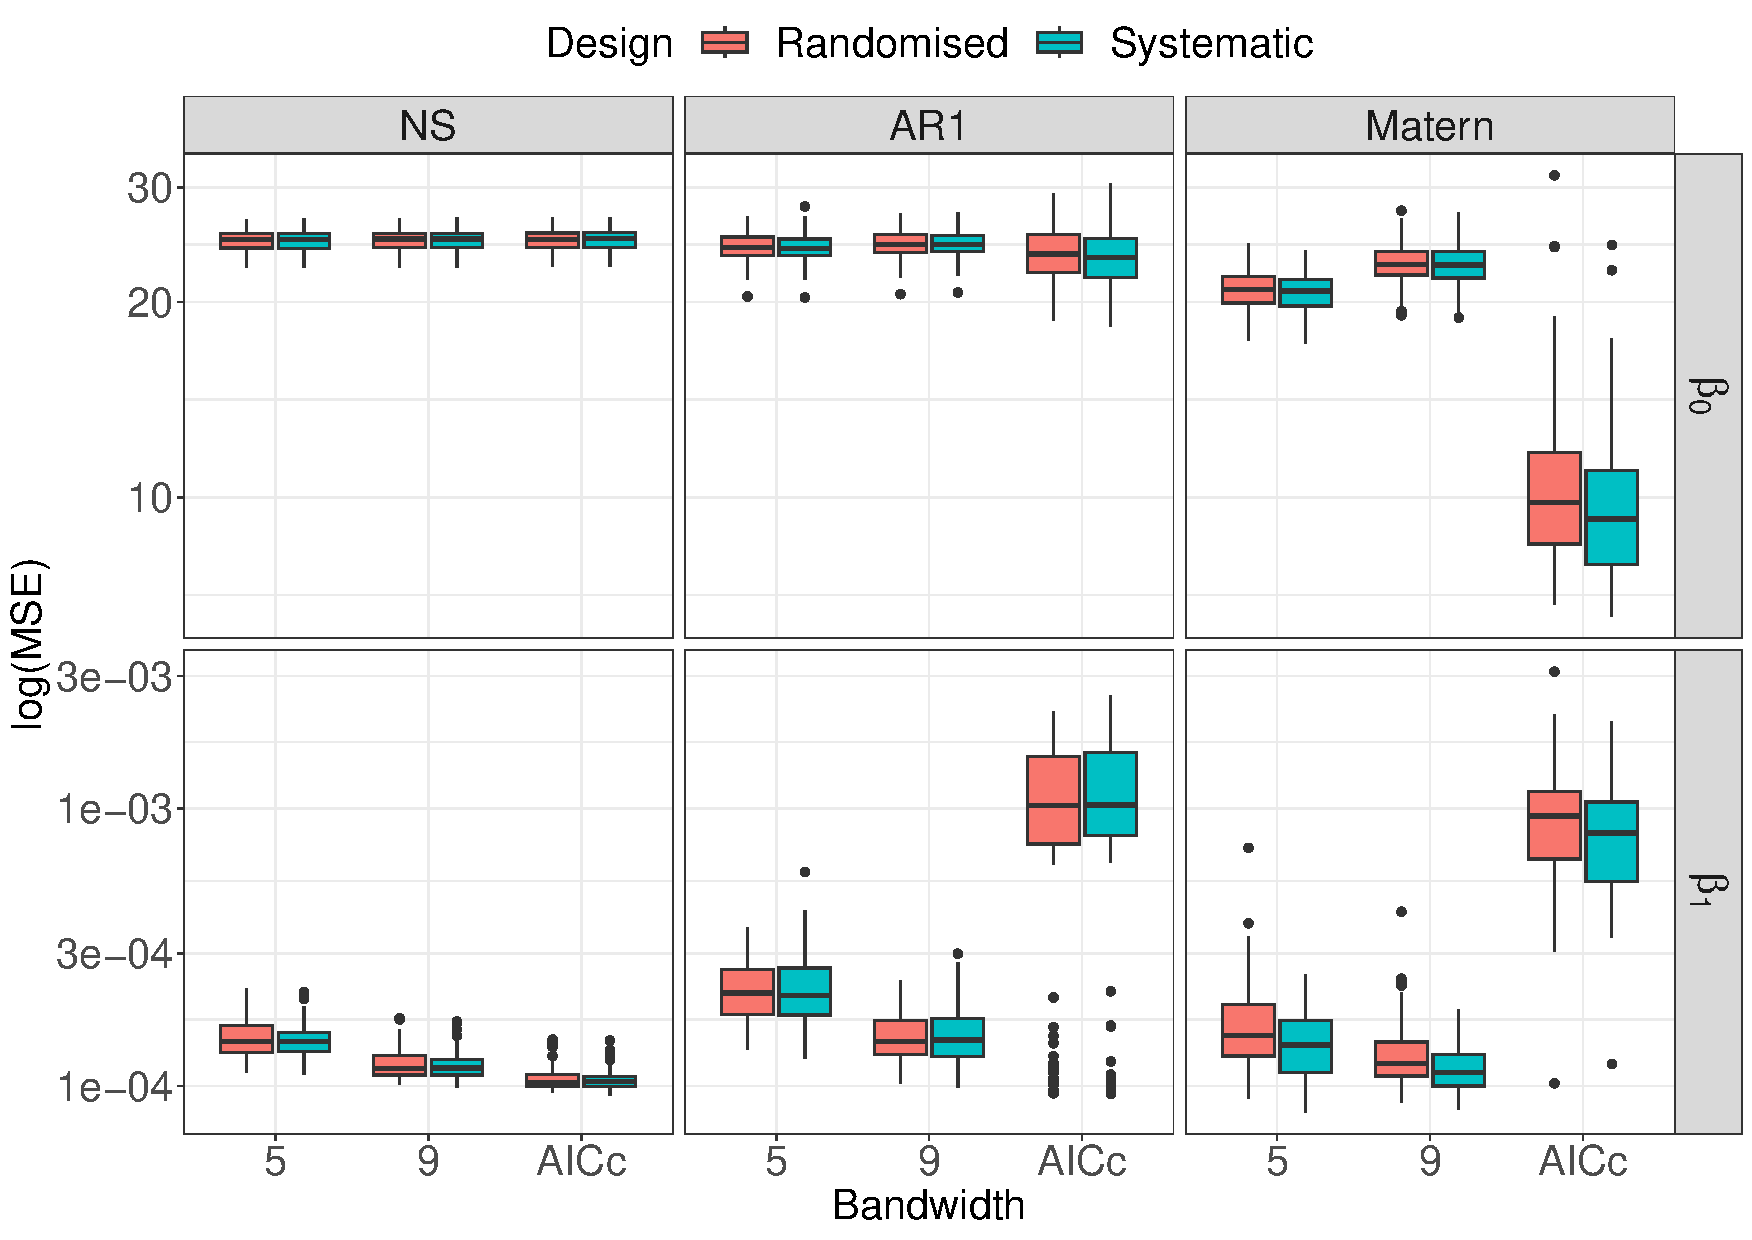
\includegraphics[width=\linewidth]{Col_LinCombMSE_newpar_eta01.pdf}
	\caption{Boxplots of the logarithm of MSE for $\hat{\beta}_0$ and $\hat{\beta}_1$ in GWR models using different bandwidths for the simulated data with a linear response. The simulated data had different spatial covariance matrices (NS, AR1$\otimes$AR1 and \Matern) and a high correlation between the parameters ($\epsilon=0.1$).}\label{fig:LinBetaMSEeta01}
\end{figure}


\begin{figure}[H]
	\centering
	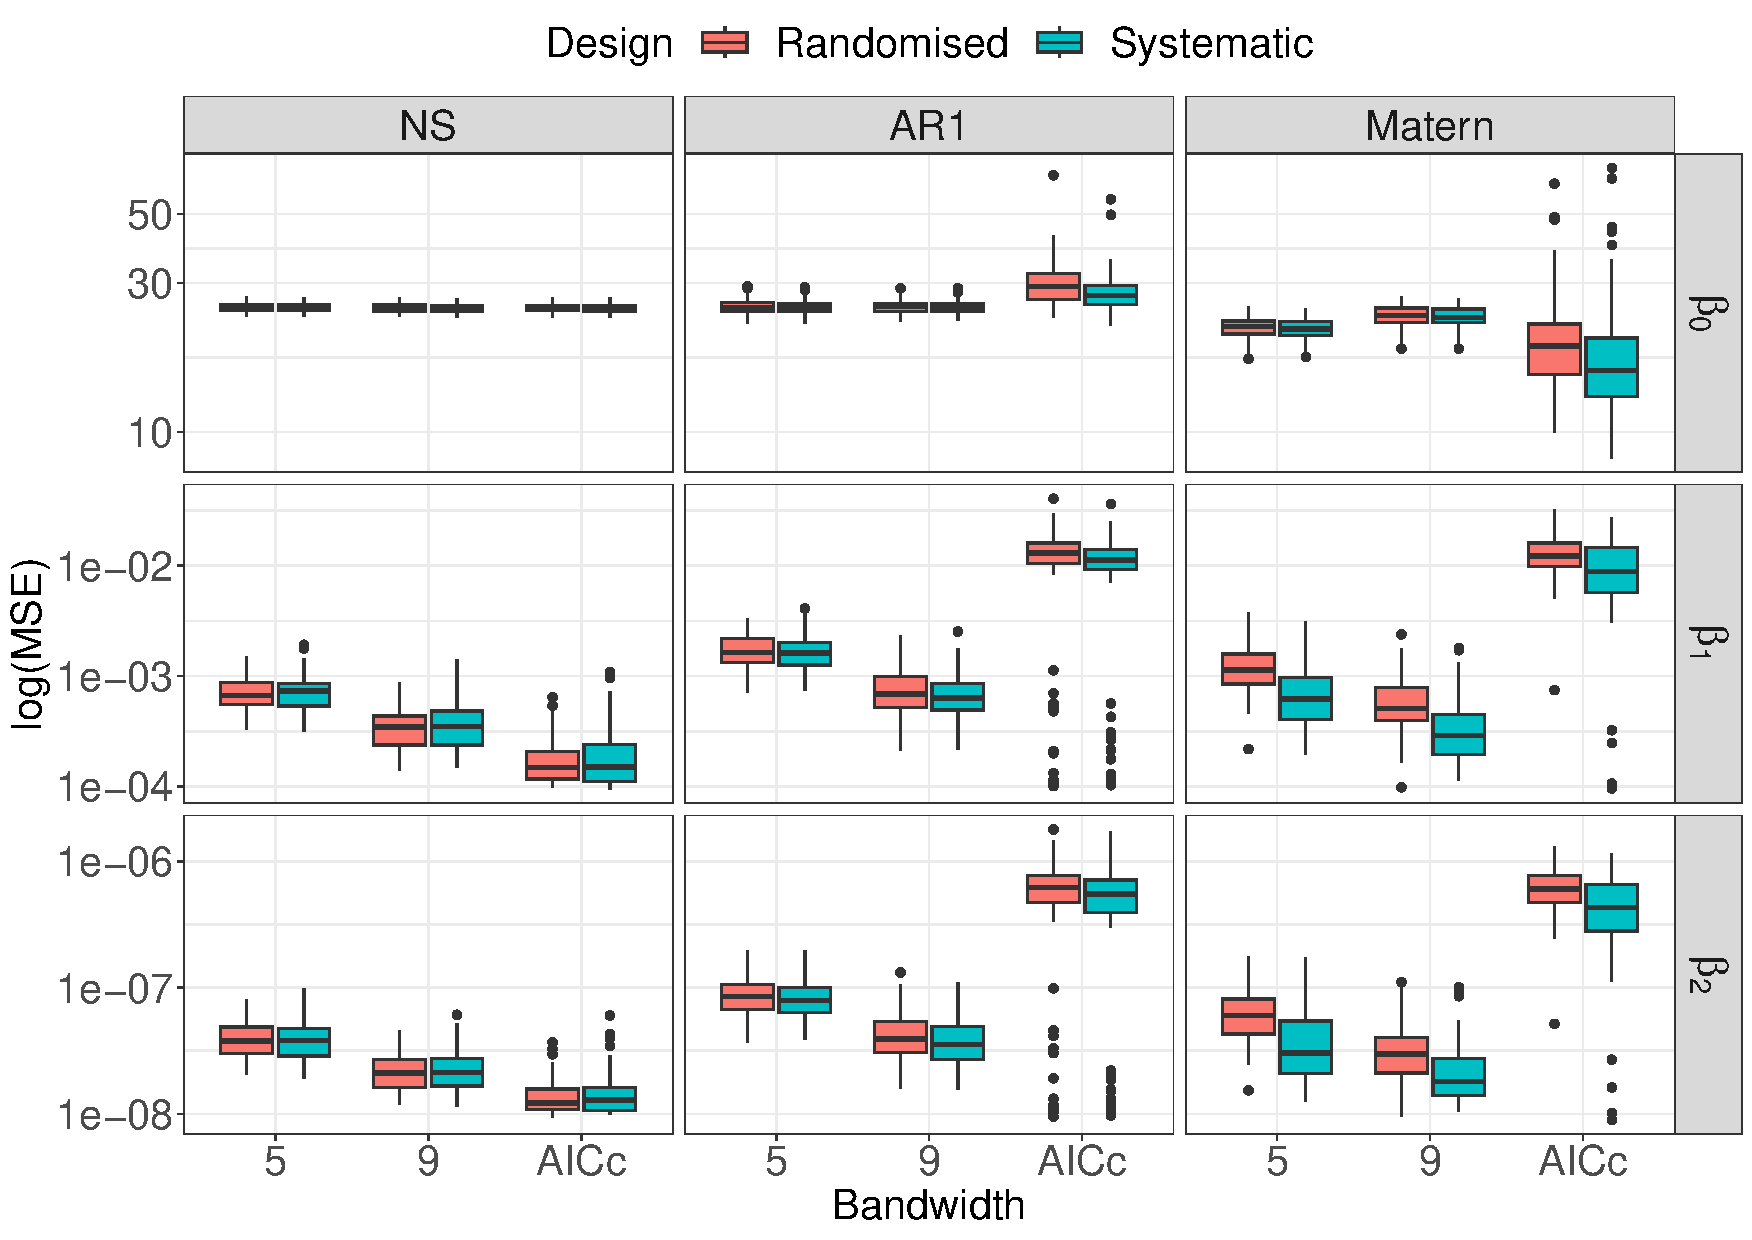
\includegraphics[width=\linewidth]{Col_QuaCombMSE_newpar_eta01.pdf}
	\caption{Boxplots of the logarithm of MSE for $\hat{\beta}_0$, $\hat{\beta}_1$ and $\hat{\beta}_2$ in GWR models using different bandwidths for the simulated data with a quadratic response. The simulated data had different spatial covariance matrices (NS, AR1$\otimes$AR1 and \Matern) and a high correlation amongst the parameters ($\epsilon=0.1$).} \label{fig:QuadBetaMSEeta01}
\end{figure}





\renewcommand\bibname{References}% change bibliography title to references
	%\addcontentsline{toc}{chapter}{Bibliography}
\addtocontents{toc}{Bibliography}
\printbibliography
\end{document}
